\documentclass[twocolumn]{article}

\usepackage{geometry}
\geometry{textwidth = 18cm,textheight = 24cm}

\usepackage{cite}
\usepackage{caption}
\usepackage{graphicx}
\usepackage{amsmath}
\usepackage{amssymb}
%\usepackage{braket}
\usepackage{textcomp}
%\usepackage{lmodern}
\usepackage{authblk}
\usepackage{datetime}
\usepackage{gensymb}
\usepackage{wrapfig}
%\usepackage[usenames,dvipsnames,svgnames,table]{xcolor}
\usepackage{booktabs}
%\usepackage{appendix}

%\usepackage[switch,columnwise]{lineno}
%\linenumbers

\newcommand{\onlinecite}[1]{\hspace{-1 ex} \nocite{#1}\citenum{#1}} 

\let\OLDthebibliography\thebibliography
\renewcommand\thebibliography[1]{
  \OLDthebibliography{#1}
  \setlength{\parskip}{0pt}
  \setlength{\itemsep}{0pt plus 0.3ex}
}
  
\title{Modeling Loop Neurons as Systems of Leaky Integrators}
%\author[1]{\Large{Saeed Khan, Alexander N. Tait, and Jeffrey M. Shainline}
\author[1]{\Large{NIST Physics and Hardware for Intelligence}
\\
\textit{\large{National Institute of Standards and Technology}}
\\
\vspace{-0.2em}
\textit{\large{325 Broadway, Boulder, CO, USA, 80305}}
\\
\vspace{-0.2em}
\textit{\large{jeffrey.shainline@nist.gov}}
}
\date{\today}%\today

\begin{document}

\twocolumn[
\begin{@twocolumnfalse}
\maketitle
\begin{abstract}

Superconducting optoelectronic loop neurons are a class of circuits potentially conducive to realizing networks for large-scale artificial cognition. These circuits employ superconducting components including single-photon detectors, Josephson junctions, and transformers. To date, all simulations of loop neurons have used first-principles circuit analysis to model the behavior of synapses, dendrites, and neurons. These circuit models are computationally inefficient and leave opaque the relationship between loop neurons and other neuron models employed in computational neuroscience and cognitive computing. Here we introduce a modeling framework that captures the behavior of the relevant synaptic, dendritic, and neuronal circuits at a phenomenological level without resorting to full solutions to the circuit equations. In this framework, each synapse and dendrite is discovered to obey a single leaky-integrator ordinary differential equation, while a neuron with adaptive refraction is modeled as two dendrites in a feedback configuration. We quantify the accuracy of the phenomenological model relative to circuit simulations, and find that the approach not only reduces the total number of differential equations in the coupled system, but also allows an increase in the numerical time step by a factor of 100. We demonstrate the use of the model with several basic examples. The net increase in computational efficiency enables future simulation of large, interconnected networks, while the formulation in terms of well-known leaky integrators provides a connection to a large body on work in applied mathematics and computational neuroscience, which aids in development of intuition for the operation of future superconducting optoelectronic networks.

\vspace{3em}
\end{abstract}
\end{@twocolumnfalse}
]

\setcounter{tocdepth}{1}
\setcounter{secnumdepth}{4}
%\tableofcontents

\section{Section}
\subsection{Subsection}
\subsubsection{Subsubsection}
\paragraph{Paragraph}

\section{\label{sec:introduction}Introduction}

% this introduction is too long-winded
Comprehensive knowledge of large-scale neural systems is a grand scientific challenge with relevance to neuroscience, artificial intelligence, and the physics of critical systems \cite{elst2012,ized2008,br2017,fama2019,eide2019}. The lack of an efficient, artificial, brain-scale experimental test bed is a barrier to progress. Experiments with living systems bring challenges, including the difficulty of obtaining data from large numbers of individual neurons, let alone synapses. Data acquired at the scale of the entire network has low resolution, while it is difficult to obtain data with high spatial and temporal resolution at the device and network levels simultaneously. The invasive nature of experiments on functioning systems is also problematic. The ability to adjust device, circuit, and network parameters of biological neural systems is limited, limiting the potential of controlled experiments. An artificial platform capable of realizing networks at the scale and complexity of the brains of intelligent organisms would be a tool of supreme scientific utility.

Neuromorphic hardware based on silicon microelectronics has a great deal to offer in this regard \cite{me1989,lide2015,chba2003,inch2006,voma2007,inli2011,cryu2012,cage2013,pfgr2013,bega2014,fu2016,moqi2018}. Yet challenges remain. Silicon neural circuits cannot directly communicate via axons in the manner of biological neurons, so communication is carried out over shared circuits comprising an interconnection network. Bottlenecks result that make information integration across space and time less efficient than biological neural systems. Additionally, adaptation and learning are hindered by difficulties with mechanisms for storing and writing a memory state in devices monolithically integrated with the MOSFETs performing neural computations. While the decades of progress developing silicon neural circuits have achieved impressive gains, as a test bed for cognition, alternative hardware may bring new benefits.

Many proposals have arisen to explore alternative hardware for cognition, including using optical \cite{psfa1985,faps1985,abps1987,waps1993,safi1995,mosc1997,hoiz2000,moho2000,rokr2009,krfo2011,dusc2012,nash2013,prsh2017,shha2017,pena2018,tafe2019} and magnetic \cite{} phenomena as well as phase-change materials \cite{chsa2019,feyo2019}. It has been argued that using optical pulses to represent action potentials may alleviate the need for a shared communication infrastructure and the associated demands on address storage and memory access \cite{shbu2017,sh2019}. The use of superconducting circuits bring the thresholding nonlinearity of Josephson junctions \cite{vatu1998,ka1999} as well as memory retention and plasticity through the storage of flux in superconducting loops \cite{sh2019}. By using superconducting detectors \cite{nata2012} in conjunction with optical pulses, neurons can signal to synapses at the single-photon level. In conjunction with minimal static power dissipation, the energy efficiency of such systems may be conducive to very large artificial cognitive systems. Although the constituent devices dwarf their biological counterparts, communication at the speed of light enables a very large neuronal pool \cite{sh2019,sh2018_ICRC}. The apparent circuit complexity and adaptability are intriguing for scientific study.

% consider starting close to here
While the components of these superconducting optoelectronic networks (SOENs) have been demonstrated, full circuits have not. Prior to undertaking the full effort and expense of realizing these complex systems, it is prudent to gain confidence they are indeed ripe for further investigation. This confidence can be gained through simulations of device, circuit, and system behavior using conventional numerical methods. The computations performed by superconducting optoelectronic loop neurons are accomplished by circuits comprising superconducting single-photon detectors, Josephson junctions, and mutual inductors. These devices are most commonly modeled with SPICE circuit simulations carried out on a picosecond time scale to accurately capture the dynamics of the Josephson junctions. Simulation of networks of large numbers of these neurons become computationally intensive. From the perspective of the neural system, the picosecond dynamics of the JJs are not the primary interest, and one would prefer to treat each synapse, dendrite, and neuron as an input-output device with a model that accurately captures the circuit dynamics on the nanosecond to microsecond time scales while not explicitly treating the picosecond behavior of the underlying circuit elements.

Here we introduce a phenomenological model of loop neurons and their constitutive elements that accurately captures the transfer characteristics of the circuits without solving the underlying circuit equations. Each synapse and dendrite is treated with a single, first-order ordinary differential equation that describes the output of the element as a function of its inputs and instantaneous internal state. These equations take the standard form of a leaky integrator with a nonlinear driving term. Each neuron performs passive summation of its synaptic and dendritic inputs. When the sum of the inputs reaches threshold, the neuron produces a spike. Refraction is treated with the same formalism as a strong inhibitory synapse receiving the neuron's spikes and directly contacting the neuron's cell body. When full circuit simulations are conducted, each synapse or dendrite require solving a system of seven equations at each time step, and time steps of 1\,ps are typical. The model presented here reduces the number of equations for each synapse or dendrite to one and allows simulation with time steps of 1\,ns. 

We begin by motivating the form of the model based on circuit considerations. We then describe the means by which the form of the driving term in the leaky integrator is obtained. Error is quantified by comparison with full circuit simulations, and convergence is investigated as a function of time step size. Point neurons are considered to test the synaptic equations. Dendrites are treated next, and the similarity between synaptic and dendritic circuits permits a treatment with a similar form of leaky integrator equation. Dendritic accuracy is quantified, and an example of a neuron with a dendritic arbor is presented to illustrate the utility of the model. Throughout the work we compare and contrast loop neurons with their biological counterparts. 

\section{\label{sec:loop_neurons}Overview of Loop Neurons}
\begin{figure}[h!]
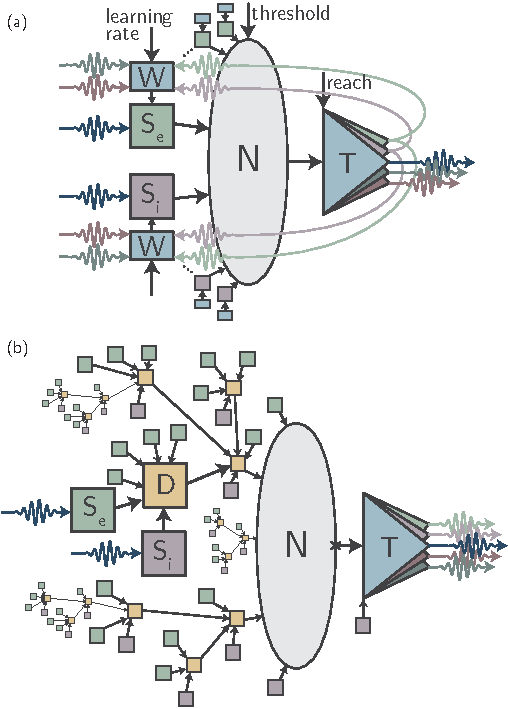
\includegraphics[width=8.6cm]{figures/_fig__schematics.pdf}
\captionof{figure}{\label{fig:schematic__circuits}Two schematics of loop neurons. (a) Schematic of a point loop neuron (no dendritic tree) \cite{sh2018,sh2019} showing excitatory ($\mathsf{S_e}$) and inhibitory ($\mathsf{S_i}$) synapses, as well as synaptic weight update circuits ($\mathsf{W}$). The wavy, colored arrows are photons, and the black arrows are electrical signals. The synapses receive signals as faint as a single photon and add supercurrent to an integration loop. Upon reaching threshold, a signal is sent to the transmitter circuit ($\mathsf{T}$), which produces a pulse of photons that are sent to downstream synaptic connections. Electrical signals generated by synapses and the neuron cell body are used for synaptic weight updates. A refractory dendrite ($\mathsf{D_r}$) receives spike outputs from the neuron and provides feedback to the neuron to accomplish adaptive refraction. (b) A loop neuron with an elaborate dendritic tree \cite{sh2020}. The complex structure consists of excitatory and inhibitory synapses that feed into dendrites ($\mathsf{D}$). Each dendrite performs computations on the inputs and communicates the result to other dendrites for further processing or on to the cell body of the neuron ($\mathsf{N}$). The neuron itself acts as the final thresholding stage, and when its threshold is reached, light is produced by the transmitter ($\mathsf{T}$), which is routed to downstream synaptic connections.}
\end{figure}

Research in superconducting optoelectronic networks of loop neurons aspires to realize artificial neural systems with scale and complexity comparable to the human brain. We have introduced the concepts of loop neurons in a number of papers \cite{sh2018,sh2019,sh2020}, and we have demonstrated many of the principles experimentally \cite{buch2017,chbu2017,chbu2018,mcve2019}. Schematic diagrams of two types of loop neuron are shown in Fig.\,\ref{fig:schematic}. Figure \ref{fig:schematic}(a) shows the point-neuron concept \cite{sh2018,sh2019_jap}, while Fig.\,\ref{fig:schematic}(b) shows the concept when a dendritic tree is included \cite{sh2019_jstqe}. In these neurons, integration, synaptic plasticity, and dendritic processing are implemented with inductively coupled loops of supercurrent. It is due to the prominent role of superconducting storage loops that we refer to devices of this type as loop neurons. 

Operation of loop neurons is as follows. Photons from upstream neurons are received by a superconducting single-photon detector (SPD) at each synapse. Using a Josephson junction (JJ) in parallel with an SPD, synaptic detection events are converted into an integrated supercurrent which is stored in a superconducting loop. The circuit diagram of a synapse is shown in Fig.\,\ref{fig:circuits}(a). The amount of current that gets added to the integration loop during a photon detection event is determined by the synaptic weight. The synaptic weight is dynamically adjusted by another circuit combining SPDs and JJs, and all involved circuits are analog. When the integrated current of a given neuron reaches a (dynamically variable) threshold, an amplification cascade begins, resulting in the production of light from a waveguide-integrated semiconductor light emitter. The photons thus produced fan out through a network of dielectric waveguides and arrive at the synaptic terminals of other neurons where the process repeats.

In loop neurons, a synapse consists of an SPD in parallel with a JJ (which together transduce photons to supercurrent), and a superconducting loop, which stores a current proportional to the number of detected photon arrival events. This loop is referred to as the synaptic integration (SI) loop. Within each neuron, the loops of many synapses are inductively coupled to a larger superconducting loop, referred to as the neuronal receiving (NR) loop, thereby inducing an integrated current proportional to a weighted sum of the currents in all the neuron's synapses. When the current in this NR loop reaches a threshold, the neuron produces a current pulse in the form of one or more flux quanta. This current is amplified and converted to voltage to produce photons from a semiconductor $p-i-n$ junction.

The currents in the synaptic and neuronal loops are analogous to the membrane potential of biological neurons \cite{daab2001,geki2002}, and the states of flux in these loops are the principal dynamical variables of the synapses and neurons in the system. Inhibitory synapses can be achieved through mutual inductors with the opposite sign of coupling. Dendritic processing can be implemented straightforwardly by adding intermediate mutually inductively coupled loops between the synaptic and neuronal loops. Synapses can be grouped on dendritic loops capable of local, nonlinear processing and inhibition. Neurons with multiple levels of dendritic hierarchy can be implemented as multiple stages of integrating loops. The temporal scales of the SI and DI loops can be set with $L/r$ time constants. I expect all synaptic and dendritic signals to leak, enabling fading memory of recent activity. Also, I hypothesize that the ability to achieve a diversity of time constants through synapses and dendrites with many $L/r$ time constants will be advantageous, and I would like to investigate this in numerical studies.

Synaptic memory is also implemented based on the stored flux in a loop, referred to as the synaptic storage (SS) loop. The state of flux in the SS loop determines the current bias to the synaptic receiver circuit discussed above. This current bias is the synaptic weight. In contrast to the SI and DI loops, the SS loop is intended to store long-term memory, and therefore I do not expect to add a resistance to this loop. If the SS loop is created with a superconducting wire of high inductance, the loop can hold many discrete states of flux, and therefore can implement many synaptic weights, if desired. Synapses with a pseudo-continuum of hundreds of stable synaptic levels between minimal and maximal saturation values are possible. Transitions between these levels can be induced based on the relative arrival times of photons from the pre-synaptic and post-synaptic neurons, thereby establishing a means for spike-timing-dependent plasticity with one photon required for each step of the memory-update process. Binary synapses are also possible, and just as we expect a diversity of $L/r$ time constants to be advantageous for tracking activity over time, we expect a diversity of synapses raging from binary to multistable to be advantageous for striking a balance between adaptability and long-term memory retention.

In the present article, we work with the component definitions introduced in Ref.\,\cite{sh2020} and reproduced here for clarity. A \textit{synapse} is a circuit that receives photons with a superconducting nanowire single-photon detector and transduces the signal to an electrical current circulating in a storage loop. Specifically, Fig.\,\ref{fig:circuits}(a) is the circuit diagram of a synapse. A \textit{dendrite} is a circuit that receives as input a signal proportional to the electrical output of one or more synapses and/or dendrites, performs a transfer function on the sum of the inputs, and produces an electrical current circulating in a storage loop as the output. Specifically, Fig.\,\ref{fig:circuits}(b) is the circuit diagram of a dendrite. A \textit{neuron cell body} receives as input a signal proportional to the electrical output of one or more synapses and/or dendrites, performs a threshold operation on the sum of the inputs, and produces as output a pulse of photons if the threshold is exceeded. Following the production of a pulse, the neuron cell body experiences a refractory period wherein threshold is temporarily significantly elevated, making subsequent pulses temporarily unlikely or impossible. The circuits that accomplish the thresholding and electrical-to-optical transduction are discussed in Refs.\onlinecite{sh2018} and \onlinecite{sh2018_full}. Based on this defintion, the components $\mathsf{N}$ and $\mathsf{T}$ in the schematic of Fig.\,\ref{fig:schematic} comprise the cell body, although it is more biologically accurate to associate the transmitter $\mathsf{T}$ in this hardware with the axon hillock of a biological neuron. 

A neuron cell body can behave similarly to a dendrite in that both can perform a nonlinear threshold function on their inputs, but in the context of the hardware under consideration we make the distinction that a dendrite produces an electrical output that is to be communicated locally, while a neuron cell body produces an optical output that is to be communicated to synapses that may be spatially distant. Additionally, dendrites are envisioned to be diverse, with different dendrites performing different transfer functions, while all neuron cell bodies are envisioned to perform only the thresholding function leading to spike production. Further, the outputs from dendrites are functions with analog amplitude and a continuous temporal envelope, while the outputs from neuron cell bodies are stereotypical spike events wherein the amplitude is intended to be constant across spikes, and the temporal envelope is intended to approximate a delta function. The amplitude of the output from a neuron cell body carries no information, and all information output from the neuron cell body is encoded in the timing of the spikes. 

The term \textit{dendritic tree} refers collectively to all the synapses and dendrites that feed into a neuron cell body. Figure \ref{fig:schematic} is intended to illustrate the potential complexity and diversity of the dendritic tree. The output optical signals from a neuron cell body reach downstream synapses through a network of dielectric waveguides, optical fibers, and free-space interconnects, as described in Refs.\,\onlinecite{sh2018_full} and \onlinecite{chbu2017,chbu2018,sh2019_ne}. These optical paths are collectively referred to as the \textit{axonal tree} and are not shown in the schematic diagram. We define a \textit{neuron} to be a system comprising a dendritic tree, a neuron cell body, and an axonal tree.

A primary goal of developing the phenomenological model presented here is to elucidate similarities and differences between loop neurons and well-studied leaky integrate-and-fire (LIF) neurons. 

%make sure to talk about speeds (max firing speed, limits, leak rates briefly mentioned)
%mention notation, superscripts refer to loops, subscripts further description or indices
%need brief summary of other superconducting neurons
\cite{clbr2006}

\section{\label{sec:leaky_integrators}Contrasting Loop Neurons with Leaky Integrate-and-Fire Point Neurons}
\begin{equation}
\label{eq:leaky_integrator}
\frac{dQ(t)}{dt} = f(t)-\frac{Q(t)}{\tau},
\end{equation}
The general form of a leaky integrator differential equation is given in Eq.\,\ref{eq:leaky_integrator}. Equation \ref{eq:leaky_integrator} models many physical systems wherein a quantity of interest, $Q$, accumulates in time due to a driving function, $f(t)$, while leaking with an exponential temporal dependence and time constant $\tau$. In neurons, the quantity of interest is the membrane potential, $V(t)$, which is due to charge on the membrane capacitance. This charge leaks exponentially due to shunt conductance between the surfaces of the membrane. The charge is provided by synapse events, which play the role of the driving function. In a point neuron model, processing in the dendritic tree is ignored, and it is assumed that the signal from all synapses is summed on the membrane, one can calculate the membrane potential on neuron $i$ with $Q(t)\rightarrow V_i(t)$ and
\begin{equation}
\label{eq:leaky_integrator__synapse_signal}
f(t) = q_0 \sum_j w_{ij} \sum_p \delta(t-t_p^{(j)}),
\end{equation}
where $w_{ij}$ is the synaptic weight, or efficacy, between neuron $j$ and neuron $i$, and $t_p^{(j)}$ is the time of the $p$th spike generated by neuron $j$.

In addition to leaky integration, a point-neuron model must produce spiking behavior and refraction. We arrive at a LIF model by supplementing Eqs.\,\ref{eq:leaky_integrator} and \ref{eq:leaky_integrator__synapse_signal} with the rule that when $V_i(t)$ reaches a threshold $V_i^{\mathrm{th}}$ from below, the neuron produces a spike, and the membrane potential is set to zero (or an appropriate reset value). While this LIF point neuron fails to capture much of the computational repertoire of biological neurons \cite{kose2000}, we recapitulate the assumptions of the model as a point of comparison for the loop neurons that are the focus of this work.

There are three distinctions to be made between the LIF model and a full loop neuron. First, loop neurons with thousands of connections are likely to employ a hierarchical dendritic tree, much like biological neurons \cite{me1994,loha2005,haah2016}, and tailored to the computational roles. Synapses store a record of their recent activity as flux in an inductive storage loop, and this signal is communicated to dendrites through transformers. Dendrites perform nonlinear operations on these signals and produce outputs as flux coupled to the next layer of the intra-neuron information-processing hierarchy. So whereas the quantity of interest in the LIF model is the membrane potential of the neuron cell body, in loop neurons the quantities of interest are the flux stored in all the synaptic and dendrite flux storage loops (the SI and DI loops discussed above).

Because the information in a loop neuron is contained in the flux storage loops the system need not be characterized by a single time constant of temporal decay. This is the second distinction between the LIF model and loop neurons. The LIF model is characterized by a single time constant determined by the rate at which charge leaks from the membrane capacitance, so a LIF neuron integrates information over a single temporal scale. By contrast, each synapse and dendrite of a loop neuron can have a distinct time constant (set by the $L/r$ time constant of the loop), so the synapto-dendritic tree of a loop neuron can integrate information across many orders of magnitude in temporal scale.

The third distinction between the LIF model and loop neurons relates to reset after production of a spike. When a LIF neuron produces a spike, its membrane potential is forced to a reset value, and all information accumulated by the neuron is discarded. By contrast, no such reset occurs in loop neurons. The cell body of the neuron receives signals from the final layer of dendrites as well as direct synapses. When the net flux from these signals drives a Josephson junction in the cell body above threshold, it produces an action potential that sends light to downstream synaptic connections. Refraction is accomplished when the signal that starts this action potential also triggers a specific dendrite that couples an inhibitory signal back to the cell body, achieving brief, negative self-feedback, which enables pulsatile behavior. Because the state of flux in the SI and DI loops is not affected by the neuron reaching threshold (with the exception of the refractory dendrite), the information contained in those loops is maintained through the firing process. 

As the subsequent sections will describe, within the framework of loop neurons, synapses behave as leaky integrators that receive delta-function temporal inputs and cumulative outputs with exponential temporal decay of nearly arbitrary time constant. Dendrites are leaky integrators as well, obeying a nearly identical differential equation to synapses. Neurons are modeled simply as a dendrite with self-feedback accomplishing refraction through another dendrite. An entire loop neuron is a network of coupled leaky integrators, the output of each given as the input to another. Communication between neurons is by optical pulse events. Thus, while a LIF point-neuron model describes a single integrator with a single leak rate, a loop neuron is itself an elaborate network of coupled integrators accumulating and leaking information across temporal scales. It is premature to conclude that a network of such complex neurons is superior to simpler LIF point neurons for information processing. The objective of this paper is to develop the mathematical model that will enable efficient simulation of large networks of loop neurons so their utility can be assessed.

\section{\label{sec:dendrites}Dendrites as Leaky Integrators}
In biological neural systems, dendrites receive inputs from synapses and other dendrites and perform nonlinear transfer functions on those inputs. The computations performed include thresholding \cite{}, logic functions \cite{}, and sequence detection \cite{}. The specific spatio-temporal function performed by biological a dendrite depends on the morphology of the dendrite itself, the location and strength of synaptic connections, and the recent history of activity \cite{}. Analogous operations can be performed by a superconducting circuit. In loop neurons, these functions are adapted through circuit parameters, some of which are set in hardware, while others dynamic through current biases. In the world of loop neurons, the basic building block of the computational infrastructure is a dendrite.

\begin{figure}[htb]
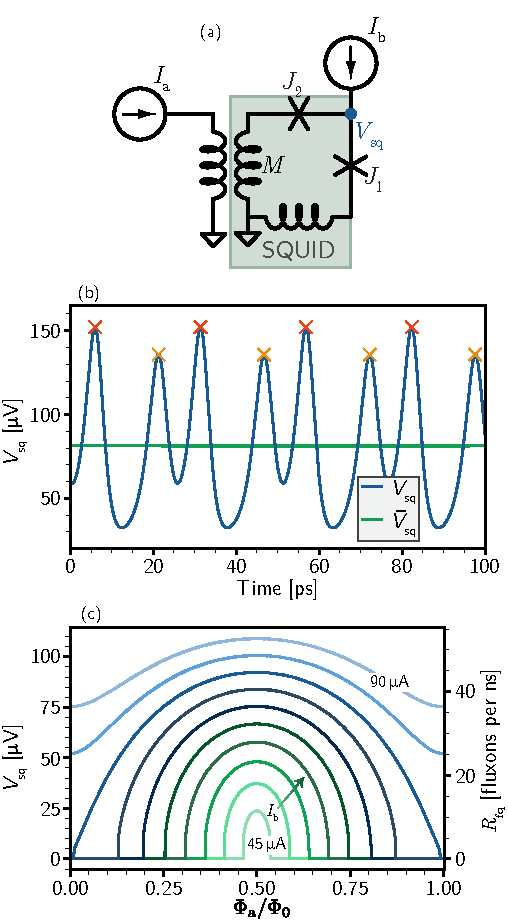
\includegraphics[width=8.6cm]{figures/_fig__dendrites__squid.pdf}
\captionof{figure}{\label{fig:dendrites__squid}Caption of fig: dendrites squid.}
\end{figure}
The core active element of superconducting electronic circuits is a Josephson junction (JJ), which comprises two superconducting leads connected by a thin barrier though which supercurrent can tunnel \cite{vatu1998,ka1999,ti1996}. A JJ can pass a current below a certain value without establishing a voltage. Above this critical current, referred to as $I_c$, the JJ will produce voltage pulses known as fluxons. These pulses carry a given current as well as magnetic flux. More detail regarding production of fluxons by a JJ is given in Appendix\,\ref{apx:dendrites_model} and in Refs.\,\onlinecite{vatu1998}, \onlinecite{ka1999}, and \onlinecite{ti1996}. To construct computational circuits, JJs work in conjunction with passive inductors, which store current and flux, as well as transformers, which couple computational blocks. 

The most ubiquitous and useful compound JJ circuit is a superconducting quantum interference device (SQUID), comprising an inductive superconducting loop with a JJ on each of the conduction pathways, as shown in Fig.\,\ref{fig:dendrites__squid}(a). The response of the circuit depends on both the direct-current bias ($I_b$), and the applied flux ($\Phi_a$) coupled through the mutual inductor ($M$). When the SQUID is driven to the voltage state, the two junctions produce fluxons in rapid succession, as shown in Fig.\,\ref{fig:dendrites__squid}(b). Note that the time between these pulses is on the order of 10\,ps, while the duration of each pulse is on the order of 1\,ps. Such speeds make JJs exciting for information processing, but present a challenge if one wishes to simulate neural circuits over durations of microseconds or longer. The rapid voltage pulses generated by the SQUID can be considered on a longer time scale as a time-averaged voltage. This time-averaged voltage, $\bar{V}_{sq}$, is shown in Fig.\,\ref{fig:dendrites__squid}(c) as a function of the applied flux, $\Phi_a$ for several values of the direct current bias, $I_b$. The rate at which fluxons are generated by the SQUID and coupled to the $L-r$ branch of the circuit is directly proportional to $\bar{V}_{sq}$. An peculiar feature of the SQUID is that response is periodic in the applied flux with period of $\Phi_0$, the magnetic flux quantum ($\Phi_0 = h/2e \approx 2$\,mV$\cdot$\,ps). The peak response occurs at $\Phi_a = \Phi_0/2$. Another important aspect of the circuit is the manner in which its response is shaped by the bias current. If the circuit is biased such that the junctions are below their critical current, a threshold quantity of flux must be applied to drive the SQUID to the voltage state, as seen in Fig.\,\ref{fig:dendrites__squid}(c). 

In the framework of loop neurons, a dendrite is a SQUID with its output fed into a flux-storage loop. The content of this loop is coupled through a transformer to drive further dendrites or the neuron cell body. Through selection of fixed circuit parameters as well as dynamic bias currents, the behavior of a dendrite can be shaped across a broad range. To predict such circuit behavior, it is common to solve circuit equations derived with the Josephson relations, which relate current and voltage to the phase of the superconducting wave function across the junction. As can be seen from the time scales in Fig.\,\ref{fig:dendrites__squid}(b), these equations must be stepped through with a 1\,ps-10\,ps time step. In the context of superconducting neurons, this time scale is the fastest in the system. Yet activity of interest will persist far longer. We would like to simulate the temporal evolution of systems with as many neurons as possible, each hosting a complex dendritic tree, over as long of time spans as possible. Reduction of the time step to 100\,ps-1\,ns would be helpful in this regard. To construct such a model, exact circuit equations tracking the superconducting phase cannot be employed. The circuit must be represented as a more abstract element.

\begin{figure*}[t]
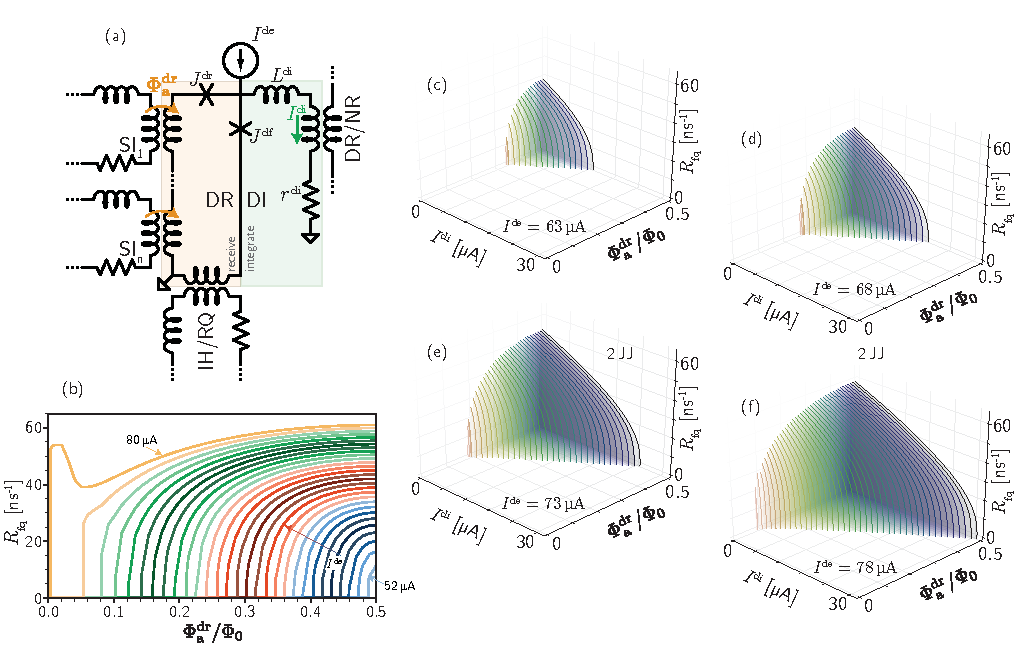
\includegraphics[width=17.2cm]{figures/_fig__dendrites__circuits__responses__2jj.pdf}
\captionof{figure}{\label{fig:dendrites__circuits__responses__2jj}Caption of fig:dendrites circuits responses 2jj.}
\end{figure*}
The objective of this section is to express the output of a dendrite as a function of the input without solving the explicit circuit equations. We would like to capture the behavior of each dendrite with a single ODE, rather than a system of coupled ODEs which is required to exactly model the circuit. We would also like to enable the ODE to be stepped through in time with as large a time step as possible, rather than requiring simulation on the picosecond time scale as required to accurately capture the dynamics of the Josephson junction. The dendrite circuit under consideration is shown in Fig.\,\ref{fig:dendrites__circuits__responses}(a), with a slightly modified version in Fig.\,\ref{fig:dendrites__circuits__responses}(b). We refer to the SQUID loop as the dendritic receiving (DR) loop and the output storage loop as the dendritic integration (DI) loop. These circuits can be modeled with a leaky-integrator equation, where the quantity being integrated and leaking is the current circulating in the DI loop, $I^{\mathrm{di}}$. The DR loop produces fluxons at a rate determined by the applied flux and the current bias, these fluxons are accumulated in the DI loop, and this integrated signal leaks with time constant $\tau_{\mathrm{dr}} = L_{\mathrm{dr}}/r_{\mathrm{dr}}$. This exponential decay is straightforward to model. The content of the storage loop feeds back to the SQUID in a negative manner, providing a saturating nonlinearity. This nonlinearity is more difficult to model. To formulate the behavior as a leaky integrator, the primary challenge is to construct the input drive term, analogous to $f(t)$ in Eq.\,\ref{eq:leaky_integrator}, which captures the positive response to flux coupled into the DR loop as well as the negative feedback when the DI loop approaches saturation.

%\begin{figure*}[t]
%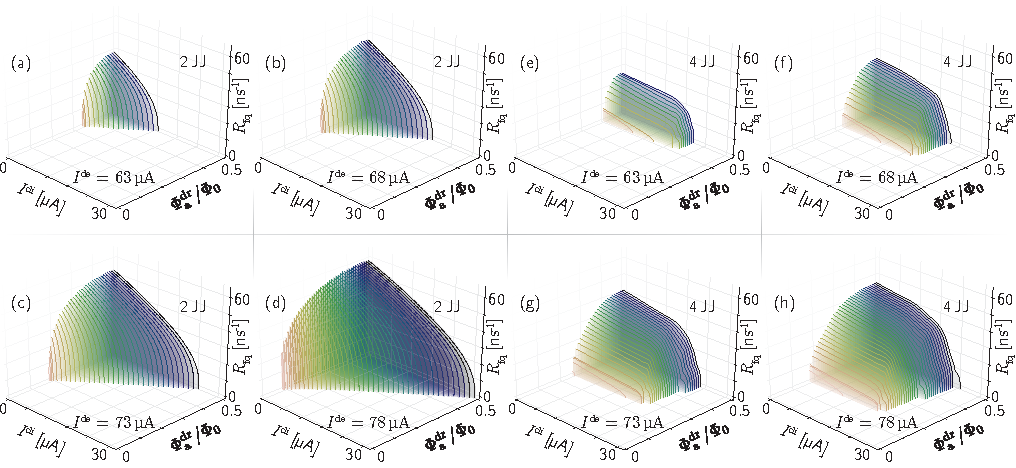
\includegraphics[width=17.2cm]{figures/_fig__dendrites__rate_arrays.pdf}
%\captionof{figure}{\label{fig:dendrites__circuits__responses}Caption of fig: dendrites rate arrays.}
%\end{figure*}
In the present work, we construct the drive term as the rate at which fluxons are added to the storage loop as a function of the input flux and the current integrated in the storage loop: $f(t)\rightarrow R_{\mathrm{fq}}(\Phi_a^{\mathrm{dr}},I^{\mathrm{di}})$. The temporal rate of change of current in the DI loop is given by
\begin{equation}
\label{eq:dendrites__leaky_integrator}
\frac{dI^{\mathrm{di}}(t)}{dt} = I_{\mathrm{fq}}\,R_{\mathrm{fq}} \left( \Phi^{\mathrm{dr}}_a(t),I^{\mathrm{di}}(t) \right) - \frac{I^{\mathrm{di}}(t)}{\tau^{\mathrm{di}}}.
\end{equation}
$R_{\mathrm{fq}} \left( \Phi^{\mathrm{dr}}_a(t),I^{\mathrm{di}}(t) \right)$ is the rate function, and $\Phi^{\mathrm{dr}}_a(t)$ is the total applied flux to the dendritic receiving loop:
\begin{equation}
\label{eq:dendrites__applied_flux}
\Phi^{\mathrm{dr}}_a(t) = \sum_i M_i I_i^{\mathrm{si/di}}(t).
\end{equation}
The sum runs over all inputs to the dendritic receiving loop, and the superscript notation $I_i^{\mathrm{si/di}}$ indicates that inputs may be from synaptic or dendritic integration loops.

The function $R_{\mathrm{fq}} \left( \Phi^{\mathrm{dr}}_a(t),I^{\mathrm{di}}(t) \right)$ represents the rate at which fluxons are added to the DI loop as a function of the total applied flux to the DR loop ($\Phi^{\mathrm{dr}}_a$), as well the current circulating in the DI loop, $I^{\mathrm{di}}$. $R_{\mathrm{fq}}$ has dimensions of fluxons per second. $I_{\mathrm{fq}} = \Phi_0/L^{\mathrm{di}}$ is the current added to the DI loop with each fluxon (described in more detail below), and has dimension of amperes per fluxon. The flux-induced current $I^{\mathrm{di}}$ circulates in the DI loop in a manner that counters the bias to $J^{\mathrm{di}}$. This counter-biasing that occurs as current accumulates in the DI loop is a form of self-feedback, which has the effect of limiting the total current that can be added to the DI loop. This saturation effect is a nonlinearity that leads to saturation in the dendritic response in a manner that is functionally similar to short-term synaptic plasticity when a synapse is coupled into the dendrite \cite{sh2020}.

The dendrite model requires specification of the form of the function $R_{\mathrm{fq}}$. There are several methods to obtain this function, and for the reasons explained in Appendix\,\ref{apx:dendrites_model}, we employ a purely numerical technique based on circuit simulations. In brief, a series of time-domain circuit simulations are conducted to obtain a lookup table for $R_{\mathrm{fq}}$ at discrete values of $\Phi^{\mathrm{dr}}_a$ and $I^{\mathrm{di}}$. These rate arrays are shown in Fig.\,\ref{fig:dendrites__circuits__responses}(c) and (d). A small number of circuit simulations is required to construct these lookup tables, and they are applicable to arbitrary values of $L^{\mathrm{di}}$ and $r^{\mathrm{di}}$ as well as the entire dynamic range of $I^{\mathrm{de}}$. These arrays are accessed when stepping through Eq.\,\ref{eq:dendrites__leaky_integrator} in time, thereby replacing the differential equations that would otherwise be required, and enabling utilization of temporal resolution on the order of 100\,ps - 1\,ns when simulating the dendritic response rather than the 1\,ps - 10\,ps time step commonly used when simulating JJs.

The rate arrays presented in Fig.\,\ref{fig:dendrites__circuits__responses}(c) and (d) elucidate the response of the circuits. Several qualitative aspects of these responses merit discussion. A primary feature of the rate arrays that plays an important role in synaptic, dendritic, and neuronal operation is the presence of a threshold value of applied flux below which the rate of fluxon production is zero and above which the SQUID activates, and the dendrite begins to accumulate signal in the DI loop. In most applications of SQUIDs, the device is used as a sensitive detector of magnetic flux, so the SQUID is biased in a voltage state, either just above threshold or at the point of maximum slope in the response curve. When used as a neural component, the SQUID comprising the DR loop of the dendrite can be biased below threshold, providing a nonlinear response function with a threshold below which weak signals evoke zero response as well as the saturating behavior of the SQUID as the signal reaches $\Phi_0/2$. The inductive inputs to the DR loop can be chosen so the net flux just reaches this maximum level when all the inputs have reached saturation. Biasing the DR loops below threshold also has the advantage of zero static power dissipation. The specific bias point, and therefore threshold, of each dendrite plays a key role in the response function. The set of all these biases can be dynamically reconfigured based on network activity, leading to the ability for adaptation and learning.  

First consider the relationship between the dendrite of Fig.\,\ref{fig:dendrites__circuits__responses}(a) to the SQUID of Fig.\,\ref{fig:dendrites__squid}. The differences are that the dendrite takes multiple inputs, and, more consequentially, in the dendrite the output is coupled to the DI loop, which integrates and leaks the accumulated flux. Cross sections of the rate array in the $\Phi^{\mathrm{dr}}_a$ - $R_{\mathrm{fq}}$ plane with small values of $I_{\mathrm{di}}$ follow the sinusoidal response seen from the SQUID in Fig.\,\ref{fig:dendrites__squid}(c). However, as current accumulates in the DI loop, the feedback effect is pronounced. For a given value of $\Phi^{\mathrm{dr}}_a$, the rate begins high and gradually decays to zero as a function of $I^{\mathrm{di}}$, with an abrupt cessation at a saturation value $I^{\mathrm{di}}_{\mathrm{sat}}$. The important distinction between the two-junction dendrite and the four-junction dendrite is that $I^{\mathrm{di}}_{\mathrm{sat}}$ is a strong function of $\Phi^{\mathrm{dr}}_a$ in the two-junction case, while $I^{\mathrm{di}}_{\mathrm{sat}}$ is nearly independent of $\Phi^{\mathrm{dr}}_a$ in the three-junction circuit. This feature allows the total signal that can be accumulated in the DI loop to be nearly decoupled from the drives to the DR loop (including the applied flux, $\Phi^{\mathrm{dr}}_a$, as well as the dendritic bias current, $I^{\mathrm{de}}$). By separating the current bias to the dendrite receiving loop, $I^{\mathrm{def}}$, from the current bias to the integration loop, $I^{\mathrm{sc}}$, the circuit decouples the threshold from the storage capacity. With the two-junction dendrite, a weak drive leads to a low value of $I^{\mathrm{di}}_{\mathrm{sat}}$, regardless of the duration of the applied signal. By contrast, a weak drive into the four-junction dendrite can lead to a large integrated current in the DI loop (large $I^{\mathrm{di}}_{\mathrm{sat}}$), provided $I^{\mathrm{sc}}$ is large and the flux drive is applied for sufficiently long. Like any leaky integrator, the accumulated signal will depend on the relationship between the drive term and the leak rate. Both the two-junction and four-junction dendrites are leaky integrators. The only difference is the form of the drive term, $R_{\mathrm{fq}}$.  

\begin{figure}[h!]
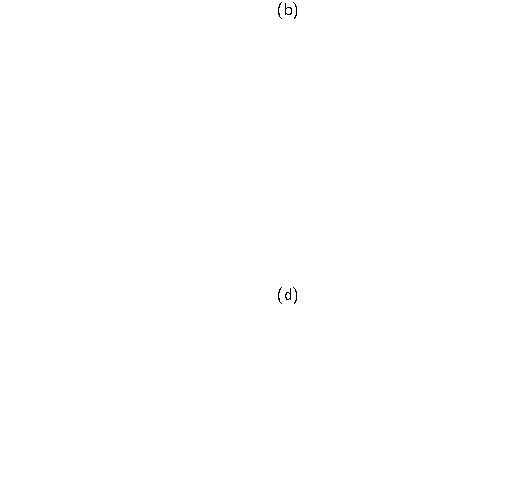
\includegraphics[width=8.6cm]{figures/_fig__dendrites__comparison__2jj__main.pdf}
\captionof{figure}{\label{fig:dendrites__comparison__2jj__main}Caption of fig:dendrites comparison 2jj main.}
\end{figure}
To quantify the accuracy of the leaky-integrator model of dendrites, we compare to full circuit simulations conducted with WRSpice \cite{wh1991}. Calculations are carried out in the time domain for a variety of inputs to the dendrite as well as circuit configurations. Accuracy is quantified with a $\chi^2$ of the form
\begin{equation}
\label{eq:chi_squared}
\chi^2 = \frac{\int dt \left|I^{\mathrm{di}}_{\mathrm{wr}}(t) - I^{\mathrm{di}}_{\mathrm{ode}}(t)\right|^2}{\int dt \left|I^{\mathrm{di}}_{\mathrm{wr}}(t)\right|^2},
\end{equation}
where the subscripts refer to the SPICE model and the ODE model of Eq.\,\ref{eq:dendrites__leaky_integrator}, respectively. Illustrative cases are shown in Figs.\,\ref{fig:dendrites__comparison__2jj__main}. Similar data from the four-junction circuit is shown in Appendix \ref{apx:dendrites_additional_data}. %Further case studies are shown in Appendix \ref{apx:dendrites_data}. 




%In both cases, the rate of fluxon production is determined by the operating point in the rate array at a given time. 

% summarize what inputs are and where they come from as well as what control knobs are available and what each does.

%The dendrite behaves as a leaky integrator, and the rate function provides the driving term. Yet the total rate at which current is added to the DI loop is scaled by the current per fluxon, $I_{\mathrm{fq}}$, which scales inversely with the loop inductance, a parameter fixed in fabrication. With $I_{\mathrm{fq}}$ large, the saturation current, $I^{\mathrm{si}}_{\mathrm{sat}}$, at which the fluxon generation rate drops to zero, will be reached with few fluxons. Inductances can be achieved to give saturation with as few as one fluxon or as many as tens of thousands. Synapses can thus be binary or analog with high bit depth. The coarse operating point is set in hardware with the choice of SI loop inductance, and it is dynamically adjusted through plasticity circuits acting to modify $I^{\mathrm{sy}}$, and therefore the number of fluxons generated in a synapse event.

%At a fixed input flux, this rate of accumulation in the DI loop is determined by the dendritic bias current, $I^{\mathrm{de}}$, and the total integrated current in the DI loop, $I^{\mathrm{di}}$. For the two-junction dendrite, $I^{\mathrm{de}}$ affects the synaptic efficacy by determining the rate during a synapse event and by setting the saturation point, whereas in the three-junction synapse the saturation point is nearly independent of the synaptic bias current. In this case, the saturation current in the SI loop, $I^{\mathrm{si}}_{\mathrm{sat}}$, is primarily affected by the the saturation control bias current, $I^{\mathrm{sc}}$. With these two degrees of freedom decoupled, the number of fluxons generated in a synapse event is determined primarily by $I^{\mathrm{sy}}$, while the maximum signal that can be integrated at the synapse is primarily determined by $I^{\mathrm{sc}}$. In the three-junction case, a large number of weak synapse events can lead to as large of a signal as a small number of strong synapse events. This is not the case on the one-junction synapse. The computational significance of this circuit feature remains to be assessed. 


%--- from synapses
%The model depends on two factors. First, current will be added to the SI loop at a rate that depends only on the instantaneous current passing through the synaptic firing junction ($I_{\mathrm{sf}}$ through $J_{\mathrm{sf}}$). Second, the current that has been added to the SI loop will decay exponentially with time constant $\tau^{\mathrm{si}} = L^{\mathrm{si}}/r^{\mathrm{si}}$. These two factors allow us to model the temporal rate of change of current in the SI loop with a leaky integrator equation:
%
%
% 
%
%The inductance also affects the leak rate, set by $\tau^{\mathrm{si}}$ in Eq.\,\ref{eq:synapses__leaky_integrator}. Because the synaptic time constant is set by $L^{\mathrm{si}}/r^{\mathrm{si}}$, the synapse storage capacity and leak rate can be adjusted independently. Arbitrarily fast leak rates are straightforward to achieve, and long time constants are also attainable in such passive superconducting circuits. Typical values of $L^{\mathrm{si}}$ are likely to be in the range 10\,nH - 10\,\textmu H. Such large inductances are possible due to high-kinetic-inductance materials \cite{}. Resistors of 1\,m$\Omega$ require care in fabrication, but are entirely possible, making passive leak time constants of 10\,ms, and potentially longer. Such time constants may make possible dynamics on biological timescales as well as the 50\,ns time scale observed when loop neurons burst at their maximum rate. The dissipationless persistence of supercurrents due to flux stored in loops also enables long-term memory retention and plasticity of various bias currents to enable learning and homeostatic adaptation. In the leaky integrator synapse model, the time constant $\tau^{\mathrm{si}}$ determines the time scale over which information is integrated. The ability to construct systems wherein neurons can draw input from synapses with such a diversity of time constants provides an opportunity to study the role of this factor in temporal dynamics such as oscillations, synchronization, and scale-free neuronal avalanches.
%
%The leaky-integrator synapse model of Eq.\,\ref{eq:synapses__leaky_integrator} captures the functionality of the circuit with acceptable accuracy, and it provides a means to understand the operation conceptually. The interesting dynamics are captured in the rate array, which shows how the excitation due to synapse events and the synaptic bias current drives the synapse, while the integrated signal provides saturation through self-feedback. The flux resolution of the integration loop is represented by the prefactor $I_{\mathrm{fq}}$, while the integration time is set by $\tau^{\mathrm{si}}$. The available parameter space is large, and a primary goal of developing this model is to enable simulations that will determine if the resulting functionality space is also useful.
%
%In addition to these degrees of freedom, one further factor determines the magnitude and sign of the drive delivered from a synapse to a dendrite or neuron. This factor is the mutual inductance between the SI loop and the DR or NR loop. We now discuss how the current in the SI loop couples through mutual inductance to become a flux drive coupled into a receiving loop. 

%I^{\mathrm{drive}} -> I^{\mathrm{ex}}, the excitation current?

%From this perspective, we can disambiguate several factors that contribute to the total drive from a synapse to a dendrite or neuron. First, with a fixed SPD bias current, the number of fluxons generated during a synapse event is determined by the synaptic bias current, $I^{\mathrm{sy}}$ , which can adapt dynamically in response to activity. Second, the total amount of current added to the SI loop
 

%It is this counter-biasing that causes the SI loop to saturate as a function of $I^{\mathrm{si}}$. When $I^{\mathrm{si}}$ becomes sufficiently large, the fluxon generated by $J^{\mathrm{jtl}}$ does not provide enough current to drive $J^{\mathrm{si}}$ above $I_c$, and the stored flux in the SI loop must decay before subsequent synapse events can add to the integrated signal.

%We begin with the hypothesis that the circuit can be modeled as a leaky integrator, with the primary dynamical quantity being the integrated current circulating in the SI loop, and a drive term resulting from photon detection events. When the SPD receives a photon, its bias current, $I_{\mathrm{spd}}$, is diverted to the synaptic firing junction, $J_{\mathrm{sf}}$. If the combination $I_{\mathrm{spd}}+I_{\mathrm{sy}}$ exceeds the critical current of $J_{\mathrm{sf}}$, a series of fluxons will be generated. At the circuit level, $J_{\mathrm{sf}}$ will first produce a fluxon. The current from this fluxon will drive $J_{\mathrm{jtl}}$ above $I_c$, causing it to produce a fluxon. Likewise, this fluxon will drive $J_{\mathrm{si}}$ above $I_c$, and the fluxon thus produced will be added to the SI loop, increasing the value of the dynamical variable of interest. After this fluxon has increased $I_{\mathrm{si}}$, if $J_{\mathrm{sf}}$ is still being held above $I_c$ by the combination of $I_{\mathrm{spd}}$ and $I_{\mathrm{sy}}$, another fluxon will be produced and propagate through the circuit in the same manner. Depending on the strength of the synaptic weight and the flux storage capacity of the SI loop, a single synapse event may add anywhere from a few fluxons up to over one thousand fluxons to the SI loop. Each fluxon adds $\Delta I_{\mathrm{si}} = \Phi_0/L_{\mathrm{si}}$ to the circulating current in the SI loop. $\Phi_0 = h/2e \approx 2\times10^{-15}\mathrm{V}\cdot\mathrm{s}$ is the magnetic flux quantum. The current in the SI loop decays with time constant $\tau_{\mathrm{si}} = L_{\mathrm{si}}/r_{\mathrm{si}}$. Given this picture of circuit operation, we can see a path toward modeling the synapse as a leaky integrator. The driving term is determined by the rate of fluxon production, and the leak term is governed by $\tau_{\mathrm{si}}$.

%\cite{amfu1994,fudr2005,fuab2007}

%--- end from synapses




\section{\label{sec:synapses}Synapses are Dendrites}
\begin{figure}[h!]
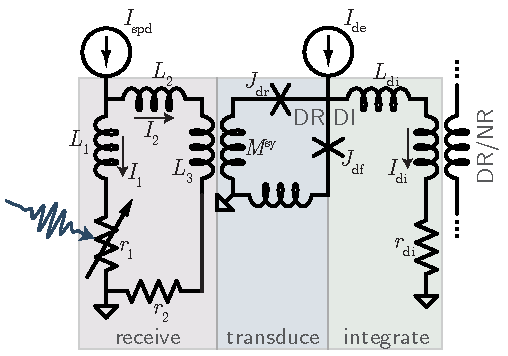
\includegraphics[width=8.6cm]{figures/_fig__synapses__circuit.pdf}
\captionof{figure}{\label{fig:synapses__circuit}Synapse circuit.}
\end{figure}

%In the world of loop neurons, a dendrite is much like a synapse, except the input current from an SPD is replaced by input flux from an SI loop, and instead of a single input, many are possible. Dendrite circuits are shown in Fig.\,\ref{fig:dendrites__circuits__responses} (a) and (b). Like the case of synapses, we consider a simple implementation where the firing junction is embedded in the flux-integration output loop as well as an extended version where the receiving loop and storage loop are separated.

%The synapse under consideration in shown in Fig.\,\ref{fig:synapses__circuits__responses}(a). In this simple form, the circuit comprises a superconducting-nanowire single-photon detector (SPD) in parallel with a Josephson junction (JJ). The JJ is embedded in a flux storage loop, referred to as the synaptic integration (SI) loop. We will also discuss a slightly more complex synapse circuit with three JJs, as shown in Fig.\,\ref{fig:synapses__circuits__responses}(b). The inputs to the circuit are photonic pulses generated by other neurons during firing events, and the output of the circuit is due to the integrated current circulating in the SI loop. This current couples flux through the mutual inductor ($M^{\mathrm{sy}}$) to a dendritic receiving (DR) loop or to the neuronal receiving (NR) loop of the cell body itself. The current bias $I^{\mathrm{sy}}$ is also an input to the circuit. This bias determines how much current is added to the SI loop with each synapse event. It is assumed that $I^{\mathrm{sy}}$ is slowly varying on the time scale of inter-spike intervals due to synaptic plasticity effects. The current bias to the SPD is assumed to be fixed for all time (at $20\,$\textmu A in this work). The critical current of all JJs considered here is $40\,$\textmu A.

%In both cases, the number of fluxons produced in a synapse event is determined by the operating point in the rate array at the moment the synapse event occurs. Assuming fixed bias to the SPD, this rate of fluxon addition to the SI loop is uniquely determined by the synaptic bias current, $I^{\mathrm{sy}}$, and the total integrated current in the SI loop, $I^{\mathrm{si}}$. For the one junction synapse, $I^{\mathrm{sy}}$ affects the synaptic efficacy by determining the rate during a synapse event and by setting the saturation point, whereas in the three-junction synapse the saturation point is nearly independent of the synaptic bias current. In this case, the saturation current in the SI loop, $I^{\mathrm{si}}_{\mathrm{sat}}$, is primarily affected by the the saturation control bias current, $I^{\mathrm{sc}}$. With these two degrees of freedom decoupled, the number of fluxons generated in a synapse event is determined primarily by $I^{\mathrm{sy}}$, while the maximum signal that can be integrated at the synapse is primarily determined by $I^{\mathrm{sc}}$. In the three-junction case, a large number of weak synapse events can lead to as large of a signal as a small number of strong synapse events. This is not the case on the one-junction synapse. The computational significance of this circuit feature remains to be assessed.

\begin{figure}[h!]
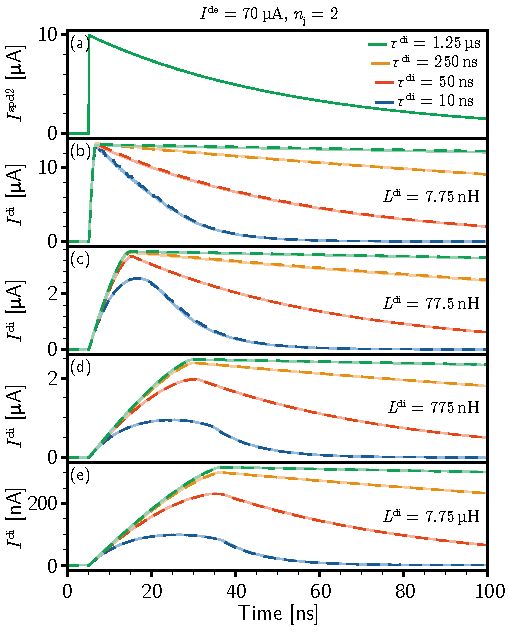
\includegraphics[width=8.6cm]{figures/_fig__synapses__comparison__2jj__single_pulse.pdf}
\captionof{figure}{\label{fig:synapses__comparison__2jj__one_pulse}synapses comparison 2jj one pulse.}
\end{figure}

\begin{figure}[h!]
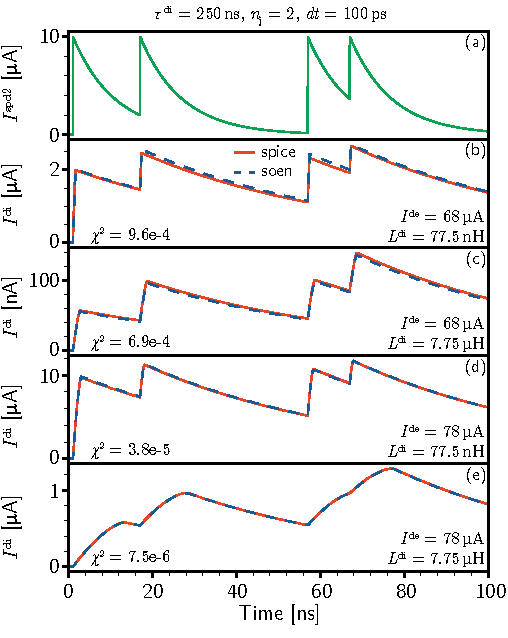
\includegraphics[width=8.6cm]{figures/_fig__synapses__comparison__2jj__pulse_sequence.pdf}
\captionof{figure}{\label{fig:synapses__comparison__2jj__pulse_sequence}synapses comparison 2jj pulse sequence.}
\end{figure}

\section{\label{sec:neurons}Neurons are Dendrites}



Here we quantify accuracy by comparing the inter-spike intervals calculated with the model to those calculated with WRSpice. For this assessment we use a $\chi^2$ of the form
\begin{equation}
\label{eq:chi_squared__ISI}
\chi^2 = \frac{ \sum_i \left| \Delta t_i^{\mathrm{ode}} - \Delta t_i^{\mathrm{wr}} \right|^2 }{ \sum_i \left| \Delta t_i^{\mathrm{wr}} \right|^2 },
\end{equation}
where $\Delta t_i$ is the inter-spike interval between spike $i$ and $i+1$. For instances wherein a single neuronal spike results from the synaptic event, accuracy is quantified as the difference in onset spike times obtained from the two calculation techniques divided by the refractory time, set by the $L/r$ time constant of the neuronal firing circuit, taken to be 50\,ns.

\begin{figure*}[h!]
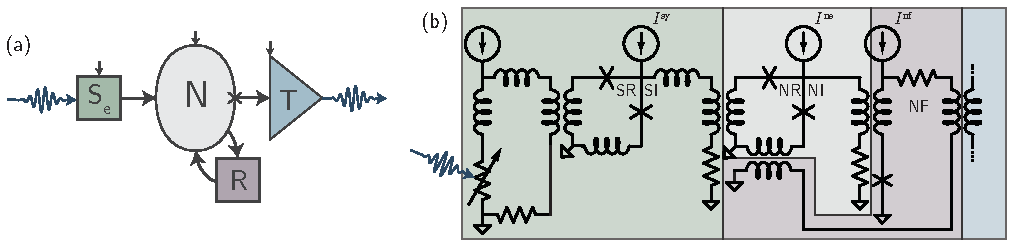
\includegraphics[width=17.2cm]{figures/_fig__neuron__one_synapse__schematic__circuit.pdf}
\captionof{figure}{\label{fig:neuron__one_synapse__schematic__circuit}Caption of fig:point neuron  one synapse  schematic  circuit.}
\end{figure*}

\begin{figure*}[h!]
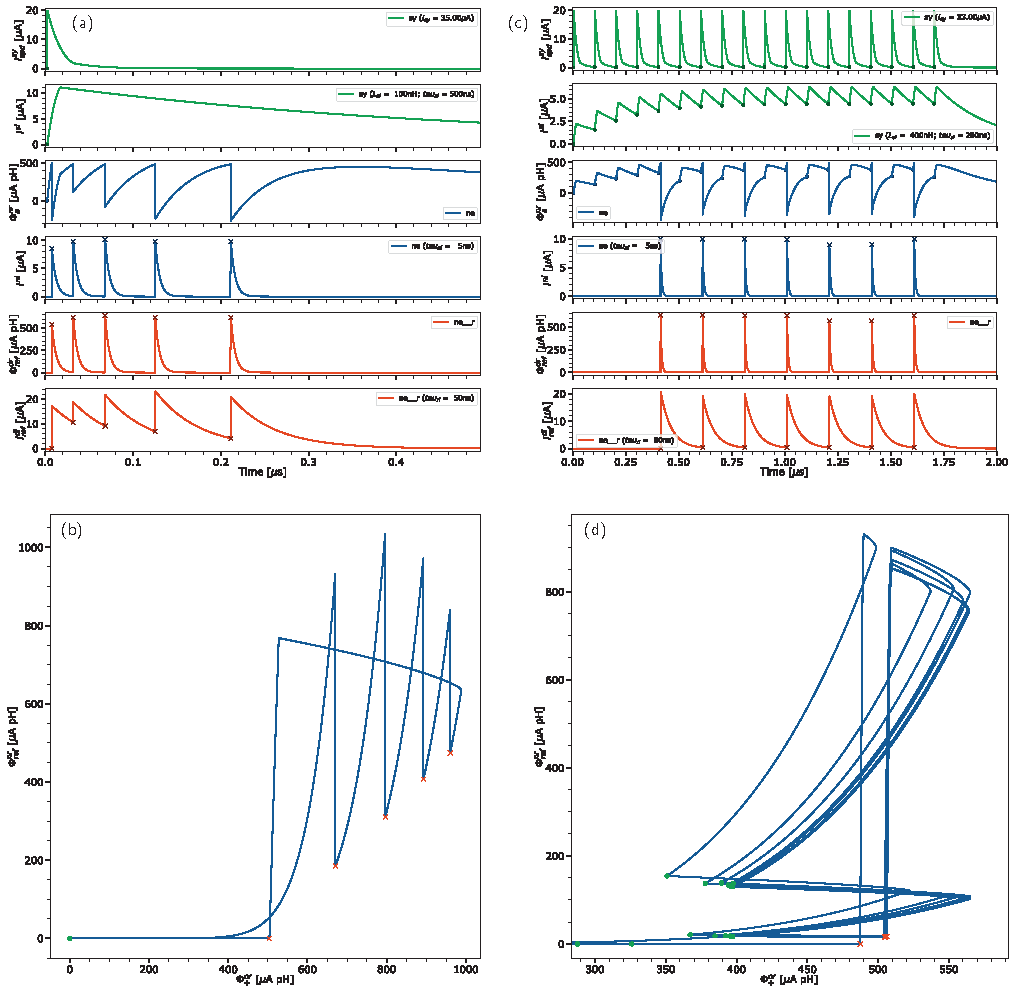
\includegraphics[width=17.2cm]{figures/_fig__neuron__one_synapse__time_traces__phase_portraits.pdf}
\captionof{figure}{\label{fig:neuron__one_synapse__data}Caption of fig:point neuron  one synapse  data. (a) Note that this type of bursting in response to a single synapse event is not possible with the synaptic reset that occurs in the standard LIF model.}
\end{figure*}

\begin{figure}[h!]
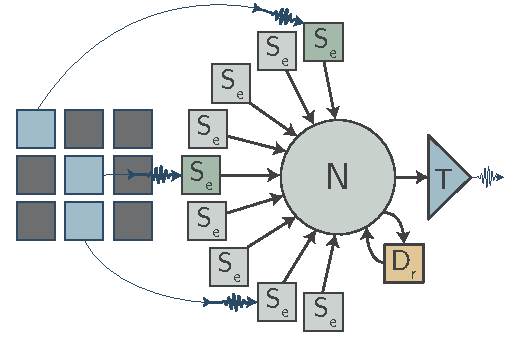
\includegraphics[width=8.6cm]{figures/_fig__neuron__nine_synapses__schematic.pdf}
\captionof{figure}{\label{fig:neuron__nine_synapses__schematic__circuit}Caption of fig:point neuron  nine  synapses  schematic.}
\end{figure}

%\begin{figure*}[h!]
%
\includegraphics[width=17.2cm]{figures/_fig__neuron__nine_synapses__data.pdf}
%\captionof{figure}{\label{fig:neuron__nine_synapses__data}Caption of fig:point neuron  nine synapses  data.}
%\end{figure*}

Need conversation of homeostatic plasticity as similar to refraction with different adaptation rate and time constant.

\section{\label{sec:discussion}Discussion: Loop Neurons are Systems of Coupled Dendrites}
We have seen that the computational circuitry of loop neurons consists of a network of interacting dendrites. Within this framework, a dendrite is a SQUID with output coupled to a flux-storage loop. The bias point of the SQUID determines the threshold input flux required to initiate activity, and the storage capacity of the output loop provides a saturating nonlinearity. The various circuit parameters provide means to adjust the response characteristics across broad operating ranges. Learning and homeostatic adaptation have not been discussed here, but the same circuits apply, dynamically adjusting bias points through coupled flux that can be stored perpetually and adjusted in small or large increments. The final stage of dendritic processing culminates in the cell body, and when this final dendrite reaches threshold, something different happens with regard to physical hardware: an amplifier drives a semiconductor light source. The threshold signal is the final stage of the computational process; the production of light is a binary action potential, and the physical transduction to photons is chosen to enable communication to many destinations across length scales. 

If the aspiration of loop neurons is to constitute systems of exceptional scale and complexity, might the simplicity of the dendritic building block limit the dynamical repertoire? We hope this model helps answer this question. It is known that even simple systems with simple rules for propagation, such as cellular automata, can give rise to behavior of great sophistication \cite{Wolfram_01}. It has been argued that similar concepts can be applied as a starting point for physics, with the rich, natural world emerging based on the interactions of fundamental nodes \cite{Wolfram_02}. Similarly, elements as simple as two-state spins interacting only with nearest neighbors (Ising model) can give rise to phase transitions and critical phenomena, including crucial long-range correlations \cite{PhaseTransitionsBooks}. By comparison, the dendrites studied here are multi-dimensional and nuanced. The nonlinear spatio-temporal convolutions occurring in each neuron's synapto-dendritic tree provide a deep repository that can inform the neuron's behavior. Transmission of action potentials to many destinations at light speed enable complex network topologies. The hierarchy of spatial connectivity in conjunction with the hierarchy of information retention times appears excellent for supporting the fractal use of space and time that supports information integration \cite{} and cognition \cite{}. Yet the simplicity of constructing the majority of computational grey matter from similar building-block components brings an advantage in modeling and technological implementation. Entire systems can be comprehended and constructed with the grasp of a one superconducting circuit and its coupling to others of its kind.

While the model presented here is interesting to explore, it is intended as a tool in a larger project. The objective of research into superconducting optoelectronic networks at this stage is to determine if SOENs are promising for future study and worthy of appreciable investment. We hope this model will help answer several questions. Do the neuromorphic circuit principles demonstrated in these superconducting optoelectronic embodiments bestow systems with the dynamic interplay of structure and function that scaffolds successful neural systems? Do device and circuit features such as diversity of time constants, high-depth synapses, the particular dendritic nonlinearities, and the available forms of plasticity bring benefits in support of criticality? Does refraction of the neuron without erasure of information in the synapto-dendritic tree offer advantages in information processing or lead to new forms of neural coding? The objective of the model presented here is to enable computational studies that answer these questions. If future work deems the hardware worthy, we hope the model can be used as a foundation for the design of more advanced technological and scientific systems.

%While photonic communication is not strictly necessary for the superconducting neural circuits discussed here, we assume it is important for achieving communication across networks of the scale at which 

%temporal hierarchy from ps JJ to ns synaptic/dendritic processes to us/ms leak/oscillations


\vspace{1em}
\section{\label{sec:acknowledgements}Acknowledgements}
\noindent This is a contribution of NIST, an agency of the US government, not subject to copyright.

\appendix

\section{\label{apx:dendrites_model}Further details regarding dendrite model}
%discuss inductances in squid loop (DR), symmetric vs asymmetric, beta_L
%discuss choice of beta_c, noise, further optimization possible
%why four-junction dendrite instead of three?

\subsection{Rate of production of fluxons by a Josephson junction}
Throughout this work, the rate function, $R_{\mathrm{fq}}$, has been obtained numerically from circuit simulations. However, it is worth considering the origin of this term with closed-form expression to the extent possible. In this subsection we present an analytical model of the one-junction synapse and explain why the model is not extensible to synapses with additional junctions or to dendrites.

This rate term in the leaky-integrator description of a superconducting optoelectronic synapse ($R_{\mathrm{fq}}$ in Eq.\,\ref{eq:synapses__leaky_integrator}) originates from well-known properties of Josephson junctions within the formalism of the resistively and capacitively shunted junction (RCSJ) model \cite{vatu1998,ka1999,ti1996}. A JJ will produce a discrete voltage pulse, referred to as a fluxon, after a time $t_{\mathrm{fq}}$ determined by the relation
\begin{equation}
\label{eq:jj__fluxon_production}
\int_0^{t_{\mathrm{fq}}} V(t) \, dt = \Phi_0.
\end{equation}
If $V(t)$ is slowly varying on the scale of $t^{\mathrm{fq}}$, we can make the approximation $V(t)\,t^{\mathrm{fq}} \approx \Phi_0$, giving the rate of fluxon generation as
\begin{equation}
\label{eq:jj__fluxon_rate}
R_{\mathrm{fq}}(t) =  \frac{1}{t_{\mathrm{fq}}} = \frac{V(t)}{\Phi_0}.
\end{equation}

An expression for $R_{\mathrm{fq}}$ can be obtained if the voltage across the synaptic firing junction is known. In the case of the one-JJ synapse, this voltage is approximately given by
\begin{equation}
\label{eq:jj__current_voltage}
V^{\mathrm{sf}}(I^{\mathrm{sf}}) = \begin{cases} V_0\left[ \left( \frac{I^{\mathrm{sf}}}{I_c-I_r} \right)^{\mu_1} - 1 \right]^{\mu_2}, & \text{for } I > (I_c-I_r)_+ \\
0, & \text{for } I < (I_c)_-
\end{cases}
\end{equation} 
The notation $I > (I_c-I_r)_+$ refers to currents $I$ that have exceeded $I_c$, driving the junction into the resistive state, and have yet to drop below $I_c-I_r$, and are therefore demonstrating hysteresis. Likewise, $I < (I_c)_-$ refers to currents that are below $I_c$ while the junction is not in the hysteretic state. $I_r = 1.1768$\,\textmu A is the reset current associated with hysteresis on $J_{\mathrm{sf}}$ due to the fact that $\beta_c = 0.95 > 0$. The values $\mu_1$, $\mu_2$, and $V_0$ depend on the specific parameters of the shunt resistance and capacitance in the RCSJ model. For the junctions considered here, fits to WRSpice data give $\mu_1 = 3.464271$, $\mu_2 = 0.306768$, and $V_0 = 233.966$\,\textmu V. From Eqs.\,\ref{eq:jj__fluxon_production} and \ref{eq:jj__current_voltage} we can obtain $R^{\mathrm{fq}}$. In the case where $I^{(\mathrm{sf})}$ is slowly varying compared to $t^{\mathrm{fq}}$, $R^{\mathrm{fq}} = V^{(\mathrm{sf})}/\Phi_0$. The voltage given by Eq.\,\ref{eq:jj__current_voltage} is only meaningful as a time-averaged approximation, and it ignores the phase of the present across the junction. 

%\begin{figure}[h!]
%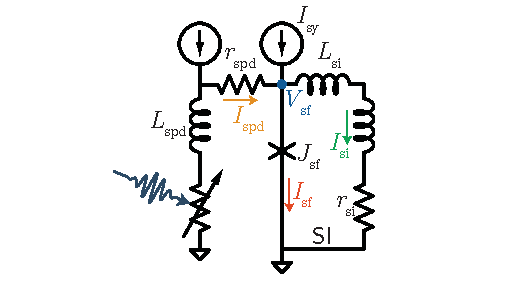
\includegraphics[width=8.6cm]{figures/_fig_apx__synapses__1jj_circuit.pdf}
%\captionof{figure}{\label{fig:apx__synapses__1jj_circuit}Caption of fig:apx synapses 1jj circuit. Need to put all correct labels in this figure (see pg 11 of green lab notebook)}
%\end{figure}
%By using the explicit form for the voltage on the synaptic firing junction, we can obtain a pair of coupled ODEs that determine the time evolution of the circuit. A labeled diagram of the circuit under consideration is shown in Fig.\,\ref{fig:apx__synapses__1jj_circuit}. The coupled ODEs are:
%\begin{equation}
%\label{eq:syn_1jj_analytical_1}
%\frac{d I^{\mathrm{si}}}{dt} = \frac{V^{\mathrm{sf}}( I^{\mathrm{sf}} - I^{\mathrm{si}} )}{L^{\mathrm{si}}} - \frac{r^{\mathrm{si}}}{L^{\mathrm{si}}} I^{\mathrm{si}},
%\end{equation}
%and
%\begin{equation}
%\label{eq:syn_1jj_analytical_2}
%\begin{split}
%\frac{d I^{\mathrm{sf}}}{dt} & = \frac{r^{\mathrm{spd1}}}{L^{\mathrm{spd}}} \left( I^{\mathrm{spd}}+^{\mathrm{sy}}-I^{\mathrm{sf}} \right) \\
%& -\frac{r^{\mathrm{spd2}}}{L^{\mathrm{spd}}} \left( I^{\mathrm{sf}}-I^{\mathrm{sy}} \right) \\
%& -\frac{1}{L^{\mathrm{spd}}} V^{\mathrm{sf}}(I^{\mathrm{sf}}-I^{\mathrm{si}}).
%\end{split}
%\end{equation}
%Note that Eq.\,\ref{eq:syn_1jj_analytical_1} is a leaky integrator ODE for the current in the SI loop, just as Eq.\,\ref{eq:synapses__leaky_integrator} in the main text. Here it is coupled to Eq.\,\ref{eq:syn_1jj_analytical_2}, which captures the current through the synaptic firing junction due to the response of the SPD as well as the current circulating in the SI loop. By stepping through Eqs.\,\ref{eq:syn_1jj_analytical_1} and \ref{eq:syn_1jj_analytical_2}, satisfactory agreement is found with SPICE circuit simulations that do not ignore the phase across the Josephson junction. However, to obtain agreement, a short time step on the order of a picosecond is required. The goals of the synaptic model are to reduce the system to a single ODE that can be stepped on a longer time scale. Simulating the model of Eqs.\,\ref{eq:syn_1jj_analytical_1} and \ref{eq:syn_1jj_analytical_2} on a 1\,ps time grid accomplishes neither of these goals. 
%
%In addition to these shortcomings of the analytical approach to a synapse model, the time-averaged approximation for the voltage across a junction (Eq.\,\ref{eq:jj__current_voltage}) provides a poor model for any circuit wherein two JJs interact with each other. Aside from the one-junction synapse, all other circuits considered in this work rely on multiple coupled JJs. In such circuits, the phases across the junctions cannot be ignored. For these reasons, we resort to numerical means of obtaining the rate functions ($R_{fq}$) for synapses and dendrites, as discussed in the following subsection.

\subsection{Determining the form of the rate function with circuit simulations}
The rate at which current is added to the SI loop depends on the total current biasing the junction ($I_{\mathrm{sf}}$), which depends on the drive ($I_{\mathrm{drive}} = I_{\mathrm{spd}}+I_{\mathrm{sy}}$) and the integrated current in the SI loop ($I_{\mathrm{si}}$). We therefore wish to form an array with values of $R_{\mathrm{fq}}$ corresponding to points in the $I_{\mathrm{sf}}$ - $I_{\mathrm{drive}}$ plane, as shown in Fig.\,\ref{fig:synapses__circuits__responses}(c). To obtain such an array, we replace the SPD and the resistor $r^{\mathrm{spd}}$ with a current source. We choose a large value for $L^{\mathrm{si}}$ so that many fluxons are required to saturate the SI loop, and we let $r^{\mathrm{si}} \rightarrow 0$ so the loop has no leak. We then simulate the circuit in time. For a given value of $I^{\mathrm{drive}}$, one obtains a list of values of $R_{\mathrm{fq}}$ as a nearly continuous function of $I^{\mathrm{si}}$ as the loop fills to saturation. With this approach, there are multiple methods of calculating the rate. One may find all voltage peaks corresponding to fluxons, and determine the time between them. Alternatively, one may track the phase across $J_{\mathrm{sf}}$ or the quantity $I^{\mathrm{si}}/I_{\mathrm{fq}}$, and differentiate with respect in time. If one wishes to calculate the rate based on fluxon times, high temporal resolution is necessary, and the output data files can become large. The rate arrays used in this work have been obtained by smoothing the quantity $I^{\mathrm{si}}/I_{\mathrm{fq}}$ with a Savitzky–Golay filter and then differentiating in time provides. By repeating this procedure for multiple values of $I^{\mathrm{drive}}$, one can build up a representation of $R_{\mathrm{fq}}(I^{\mathrm{drive}},I^{\mathrm{si}})$, as shown in Fig.\,\ref{fig:dendrites__circuits__responses}(c). In this work, we have used WRSpice \cite{wh1991} to perform the circuit simulations. The netlist was edited with Python scripts to facilitate looping over $I^{\mathrm{drive}}$.

A beneficial aspect of this method of determining the rate array is that it applies directly to the three-junction synapse as well. To obtain the rate array shown in Fig.\,\ref{fig:synapses__circuits__responses}(d), the same method of replacing the SPD with a static current source was used to construct each trace of $R_{\mathrm{fq}}$ versus $I^{\mathrm{si}}$. We have used a resolution of 250\,nA in $I^{\mathrm{drive}}$. Therefore, with this technique, roughly 40 circuit simulations are sufficient to obtain a rate array with sufficient resolution to provide the accuracy of synaptic responses presented here. Each circuit simulation captures 1\,\textmu s of simulated time, requiring $xy$\,s of CPU time. Once these simulations are run and the rate array has been constructed, it is used as a lookup table on each time step of the simulation of the synaptic ODE, Eq.\,\ref{eq:synapses__leaky_integrator}. A different lookup table must be constructed for the one-junction and three-junction circuits, but each table is applicable to a broad range of values of the circuit parameters $L^{\mathrm{si}}$, $r^{\mathrm{si}}$, and $I^{\mathrm{sy}}$. The table used in this work for the one-junction synapse is 536\,kB, while that for the three-junction synapse is 739\,kB.

One of the inputs to the rate array, $R_{\mathrm{fq}}$, is $I^{\mathrm{drive}}$, which is the sum of the synaptic bias current, $I^{\mathrm{sy}}$, and the current diverted from the SPD upon detection of a synapse event, $I^{\mathrm{spd}}$. When an SPD detects a photon, it develops a large resistive section ($\approx 5$\,k$\Omega$) for a brief duration ($\approx 200\,$\,ps) \cite{}. This resistance returns to zero once superconductivity is restored. Accurately modeling the temporal response of the current $I^{\mathrm{spd}}$ following a synapse event unfortunately requires knowledge of the voltage across $J^{\mathrm{sf}}$ on the picosecond time scale. To avoid adding this burden to our numerical scheme, we also resort to a lookup-table approach for $I^{\mathrm{spd}}$. Here we simulate the circuits of Fig.\,\ref{fig:synapses__circuits__responses}(a) and (b) with the SPD modeled as a 200\,ps, 5\,k$\Omega$ resistive segment following a detection event. We use a large SI inductance to ensure self-feedback is negligible, and we simulate the circuit for roughly 40 values of $I^{\mathrm{sy}}$ to obtain $I^{\mathrm{spd}}$ as a function of time following a synapse event. This lookup table is then used to determine the drive to $R_{\mathrm{fq}}$ following a synapse event. While this approach to determining the SPD response leads to acceptable accuracy and speed when used to simulate synapses, it is by far the least elegant aspect of the model.

\subsection{\label{apx:dendrites_additional_data}Additional Dendrite Data}


\begin{figure*}[t]
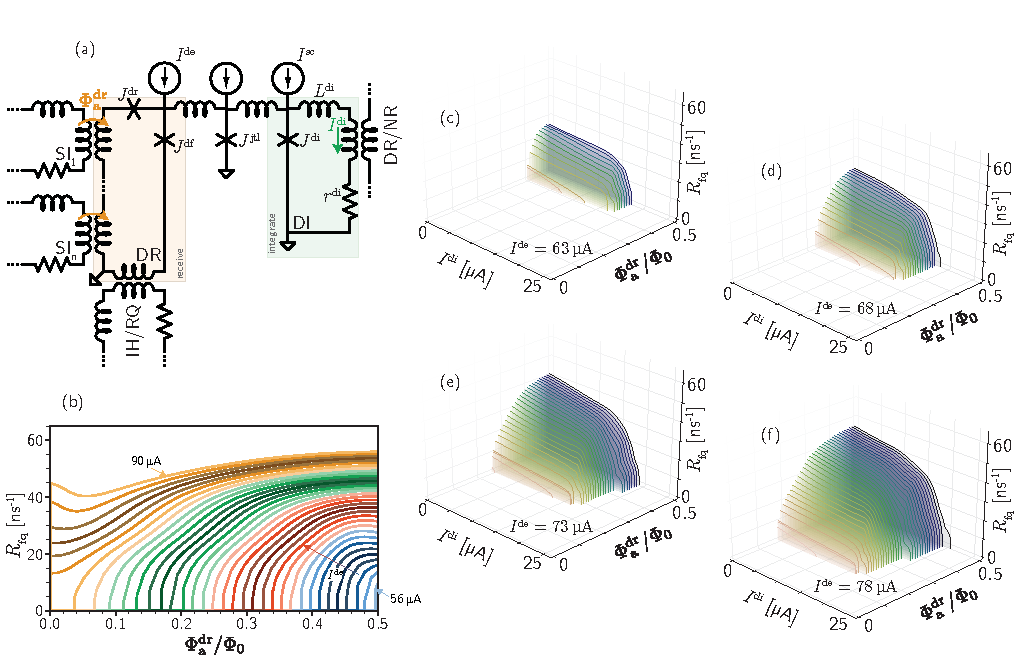
\includegraphics[width=17.2cm]{figures/_fig__dendrites__circuits__responses__4jj.pdf}
\captionof{figure}{\label{fig:dendrites__circuits__responses__4jj}Caption of fig:dendrites circuits responses 4jj.}
\end{figure*}

\begin{figure}[h!]
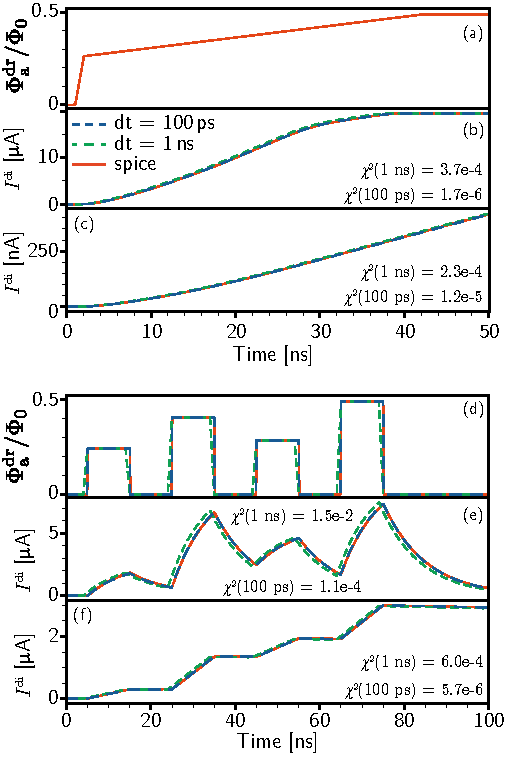
\includegraphics[width=8.6cm]{figures/_fig__dendrites__comparison__4jj__main.pdf}
\captionof{figure}{\label{fig:dendrites__comparison__4jj__main}Caption of fig:dendrites comparison 4jj main.}
\end{figure}

\begin{figure}[h!]

\includegraphics[width=8.6cm]{figures/_fig__dendrites__error_vs_dt__2jj.pdf}
\captionof{figure}{\label{fig:dendrites__error_vs_dt__2jj}dend error vs dt 2jj.}
\end{figure}

\begin{figure}[h!]

\includegraphics[width=8.6cm]{figures/_fig__dendrites__error_vs_dt__4jj.pdf}
\captionof{figure}{\label{fig:dendrites__error_vs_dt__4jj}dend error vs dt 4jj.}
\end{figure}

\section{\label{apx:synapses_model}Response of the Single-Photon Detector}
The response of the SPD circuit of Fig.\,\ref{fig:synapses__circuit} upon detection of a photon is given by
\begin{equation}
\label{eq:syn__spd_current}
I_{\mathrm{2}}(t) = \begin{cases} I_{\mathrm{spd}} \frac{r_{\mathrm{1}}}{r_{\mathrm{1}} + r_{\mathrm{2}}} \left( 1 - e^{-t/\tau_+} \right), & \text{for } 0 \le t \le t_0 \\[10pt]
I_0 e^{-(t-t_0)/\tau_-}, & \text{for } t > t_0,
\end{cases}
\end{equation} 
where
\begin{equation}
\nonumber
I_0 = I_{\mathrm{spd}}\frac{r_{\mathrm{1}}}{r_{\mathrm{1}} + r_{\mathrm{2}}}\left( 1 - e^{-t_0/\tau_+} \right),
\end{equation}
with
$\tau_+ = L_{\mathrm{tot}}/(r_{\mathrm{1}}+r_{\mathrm{2}})$ and $\tau_- = L_{\mathrm{tot}}/r_{\mathrm{2}}$. $L_{\mathrm{tot}} = L_{\mathrm{1}}+L_{\mathrm{2}}+L_{\mathrm{3}}$, and $L_{\mathrm{3}}$ is the inductor on the left side of the mutual inductor, $M_{\mathrm{sy}}$, in Fig.\,\ref{fig:synapses__circuit}. In this model, $t_0$ is the duration during which superconductivity is broken in the SPD following the absorption of a photon, which we take to be 200\,ps, following the model of Ref.\,\onlinecite{yake2007}.

\subsection{\label{apx:synapses_additional}Additional Synapse Data}

\begin{figure}[h!]
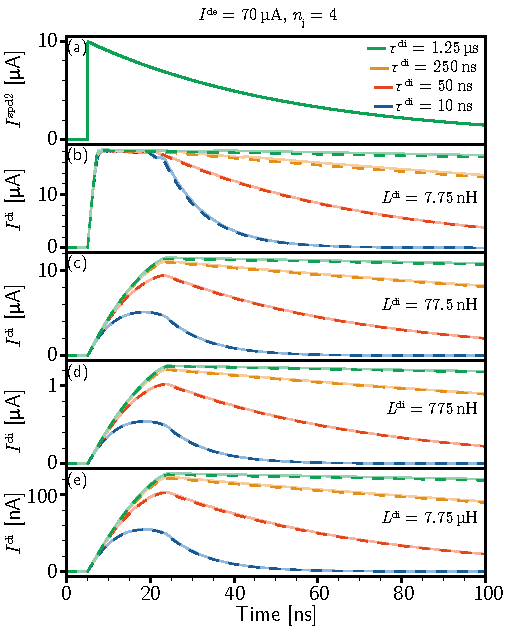
\includegraphics[width=8.6cm]{figures/_fig__synapses__comparison__4jj__single_pulse.pdf}
\captionof{figure}{\label{fig:synapses__comparison__4jj__one_pulse}synapses comparison 4jj one pulse.}
\end{figure}

\begin{figure}[h!]
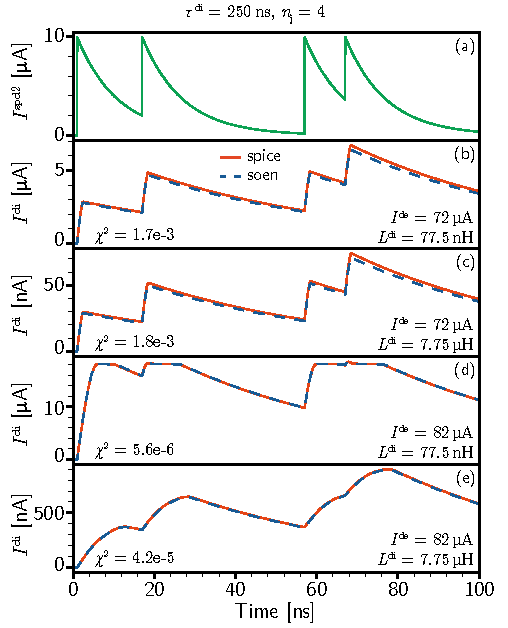
\includegraphics[width=8.6cm]{figures/_fig__synapses__comparison__4jj__pulse_sequence.pdf}
\captionof{figure}{\label{fig:synapses__comparison__4jj__pulse_sequence}synapses comparison 4jj pulse sequence.}
\end{figure}

\begin{figure}[h!]
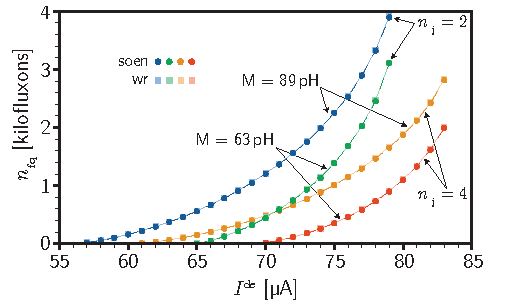
\includegraphics[width=8.6cm]{figures/_fig__synapses__nfq_vs_Ide.pdf}
\captionof{figure}{\label{fig:synapses__nfq_vs_Ide}nfq vs Ide.}
\end{figure}

%\begin{figure}[h!]
%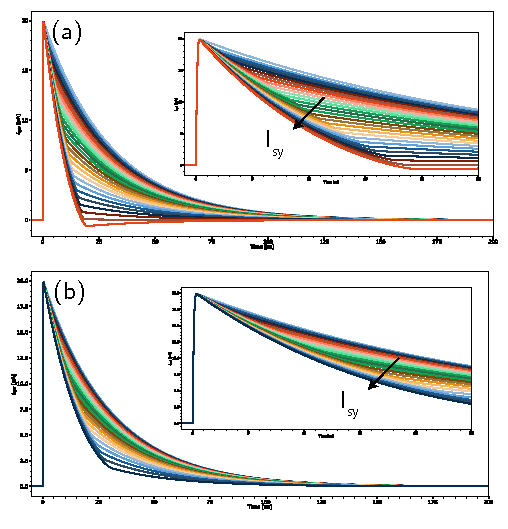
\includegraphics[width=8.6cm]{figures/_fig_apx__synapses__spd__responses.pdf}
%\captionof{figure}{\label{fig:synapses__spd_responses}Caption of fig:synapses spd responses.}
%\end{figure}
%
%\begin{figure*}[h!]
%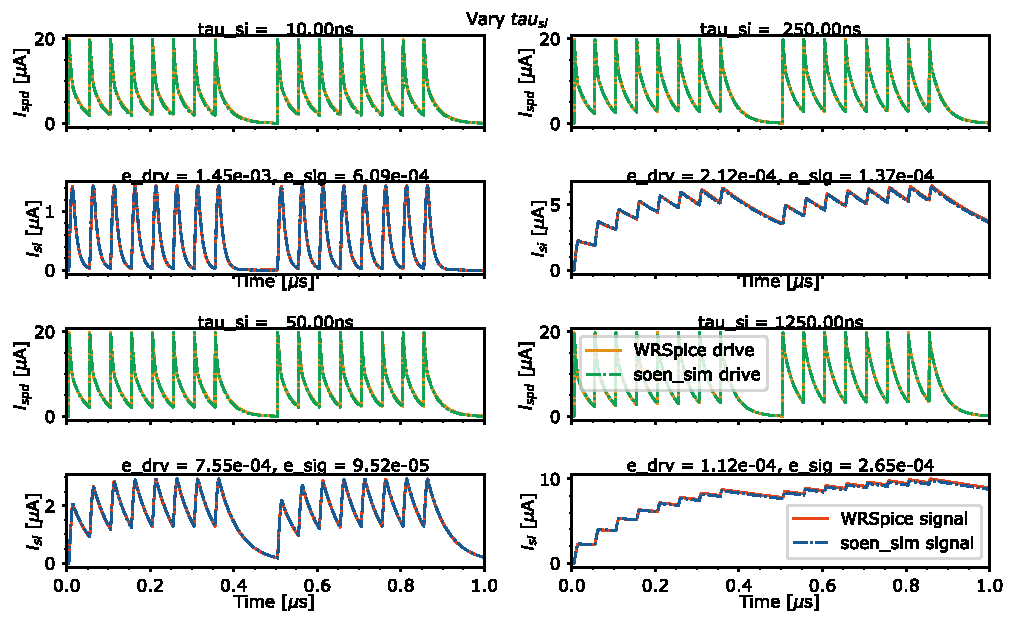
\includegraphics[width=17.2cm]{figures/_fig_apx__synapses__comparison__1jj__tau_si.pdf}
%\captionof{figure}{\label{fig:synapses__comparison__1jj__tau_si}Caption of fig:synapses comparison 1jj tau si.}
%\end{figure*}
%
%\begin{figure*}[h!]
%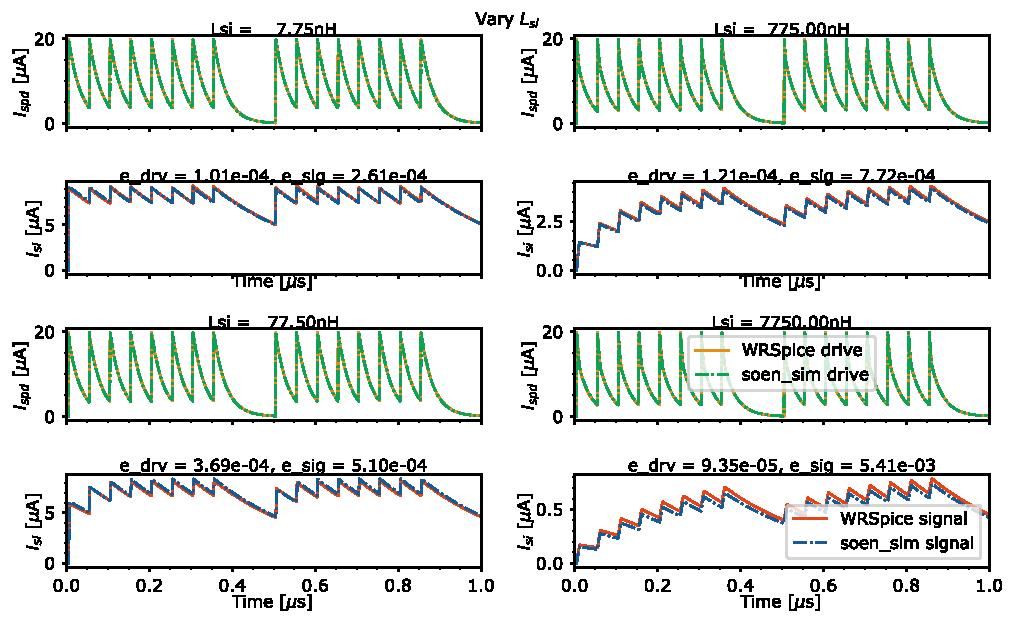
\includegraphics[width=17.2cm]{figures/_fig_apx__synapses__comparison__1jj__L_si.pdf}
%\captionof{figure}{\label{fig:synapses__comparison__1jj__L_si}Caption of fig:synapses comparison 1jj L si.}
%\end{figure*}
%
%\begin{figure*}[h!]
%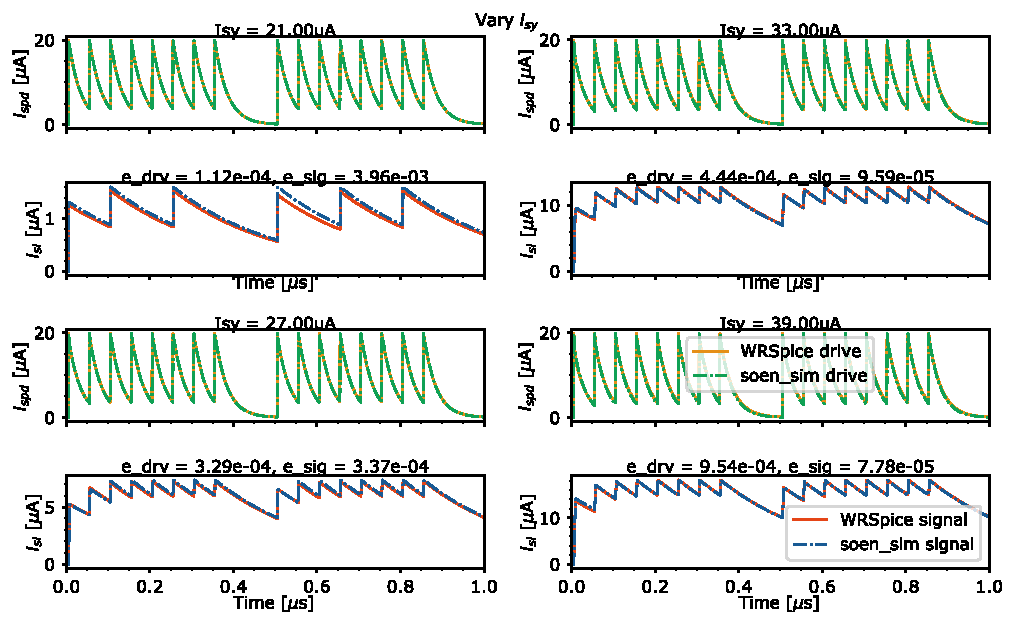
\includegraphics[width=17.2cm]{figures/_fig_apx__synapses__comparison__1jj__I_sy.pdf}
%\captionof{figure}{\label{fig:synapses__comparison__1jj__I_sy}Caption of fig:synapses comparison 1jj I sy.}
%\end{figure*}
%
%\begin{figure*}[h!]
%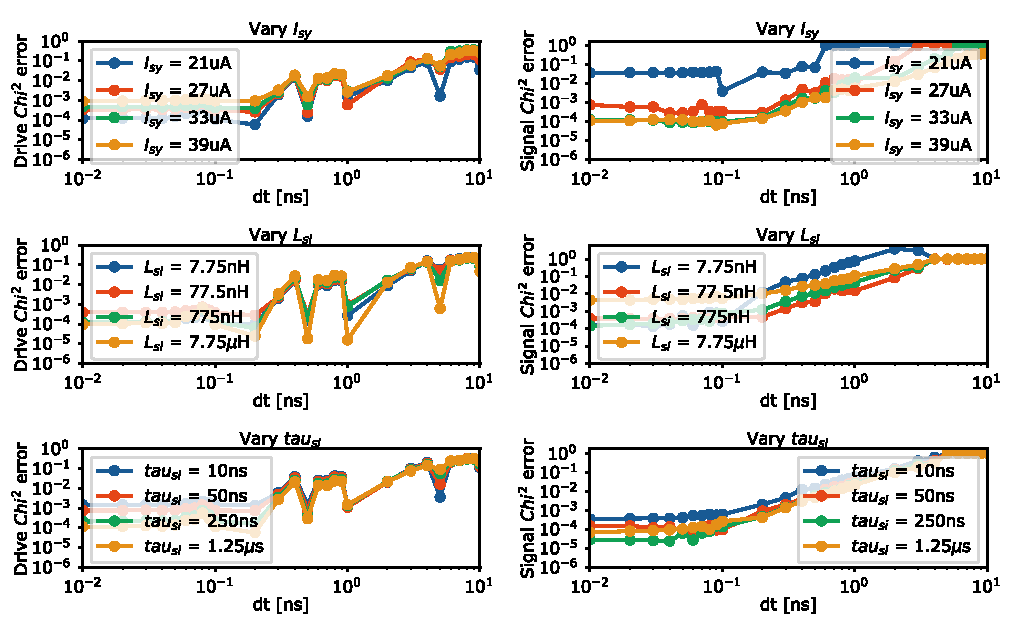
\includegraphics[width=17.2cm]{figures/_fig_apx__synapses__error_vs_dt__2jj.pdf}
%\captionof{figure}{\label{fig:synapses__error_vs_dt__2jj}Caption of fig:synapses error vs dt 2jj.}
%\end{figure*}
%
%\begin{figure*}[h!]
%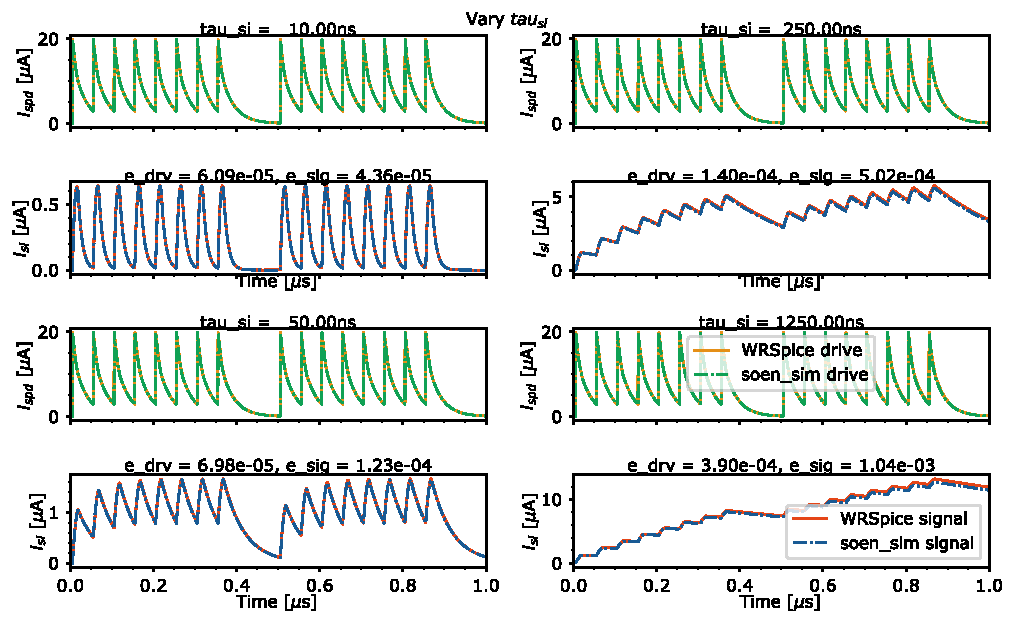
\includegraphics[width=17.2cm]{figures/_fig_apx__synapses__comparison__3jj__tau_si.pdf}
%\captionof{figure}{\label{fig:synapses__comparison__3jj__tau_si}Caption of fig:synapses comparison 3jj tau si.}
%\end{figure*}
%
%\begin{figure*}[h!]
%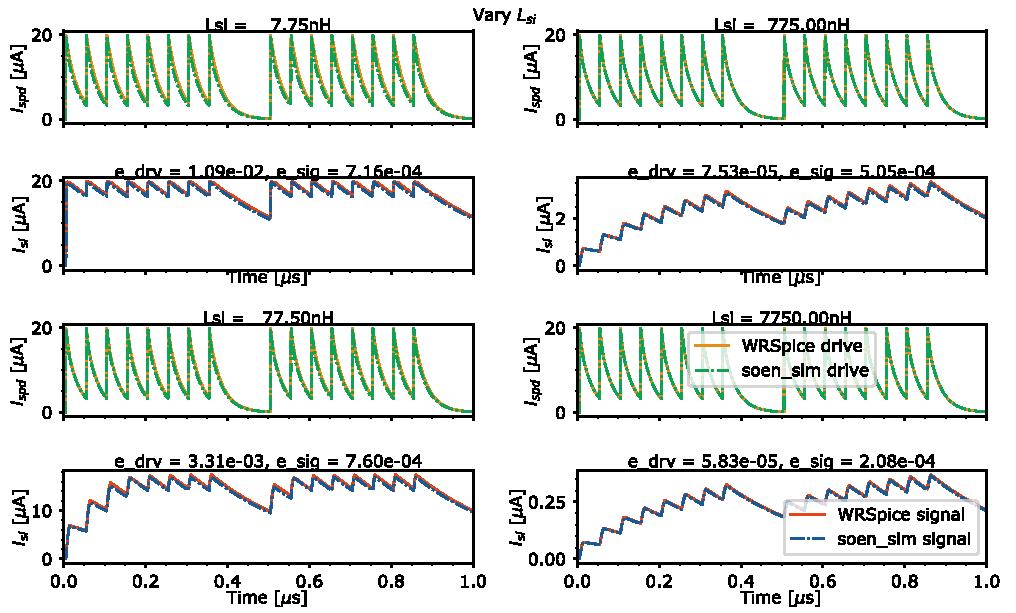
\includegraphics[width=17.2cm]{figures/_fig_apx__synapses__comparison__3jj__L_si.pdf}
%\captionof{figure}{\label{fig:synapses__comparison__3jj__L_si}Caption of fig:synapses comparison 3jj L si.}
%\end{figure*}
%
%\begin{figure*}[h!]
%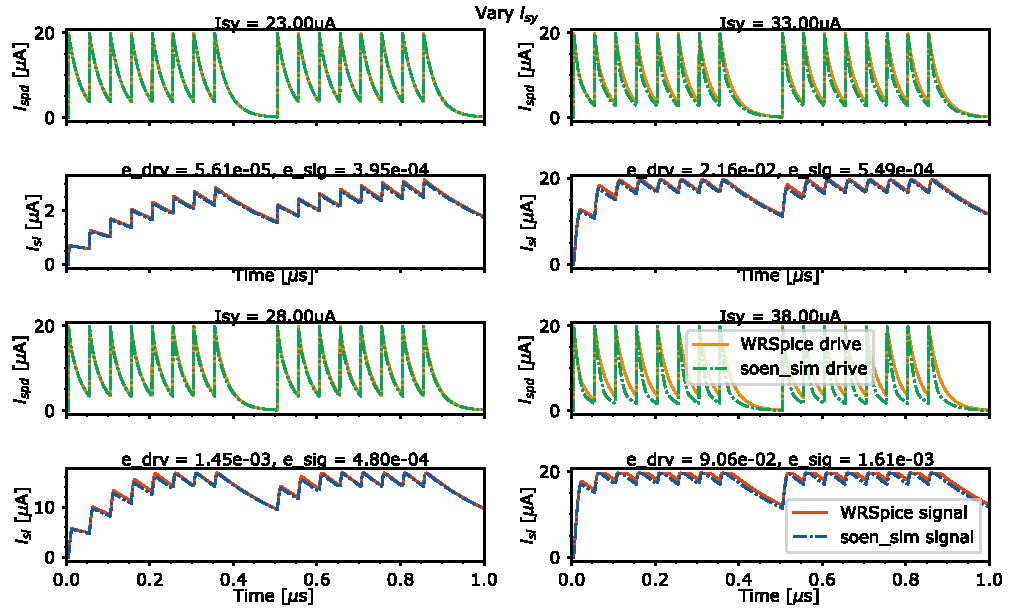
\includegraphics[width=17.2cm]{figures/_fig_apx__synapses__comparison__3jj__I_sy.pdf}
%\captionof{figure}{\label{fig:synapses__comparison__3jj__I_sy}Caption of fig:synapses comparison 3jj I sy.}
%\end{figure*}
%
%\begin{figure*}[h!]
%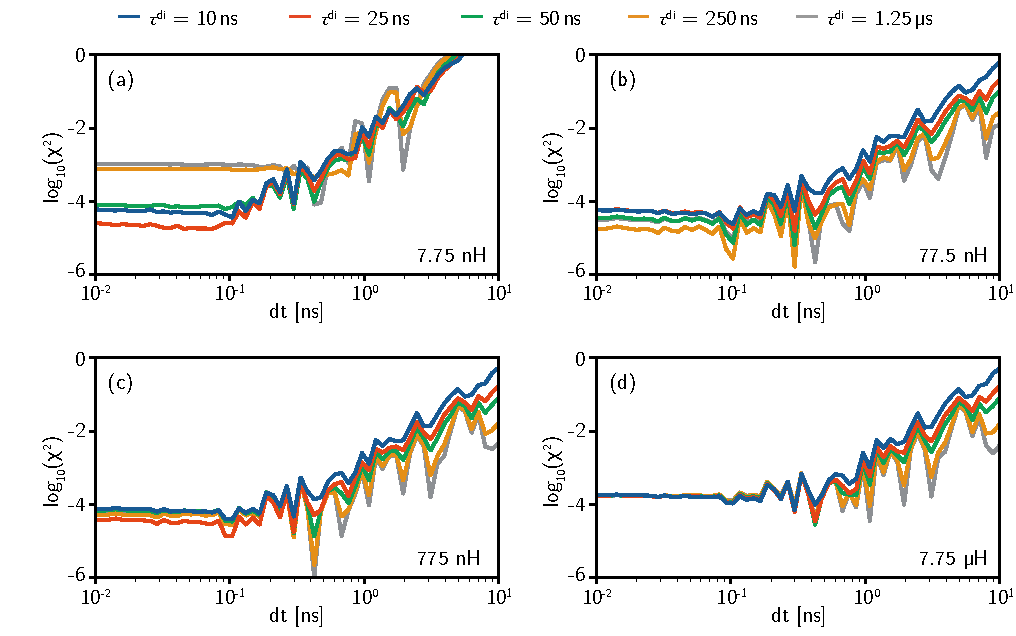
\includegraphics[width=17.2cm]{figures/_fig_apx__synapses__error_vs_dt__4jj.pdf}
%\captionof{figure}{\label{fig:synapses__error_vs_dt__4jj}Caption of fig:synapses error vs dt 4jj.}
%\end{figure*}

%\section{\label{apx:dendrites}Further data regarding dendrite modeling}

%\begin{figure}[h!]
%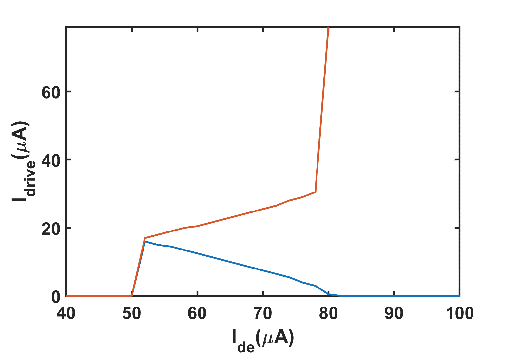
\includegraphics[width=8.6cm]{figures/_fig__dendrites__min_max__2jj.pdf}
%\captionof{figure}{\label{fig:dendrites_min_max__2jj}Caption of fig:dendrites min max 2jj.}
%\end{figure}
%
%\begin{figure}[h!]
%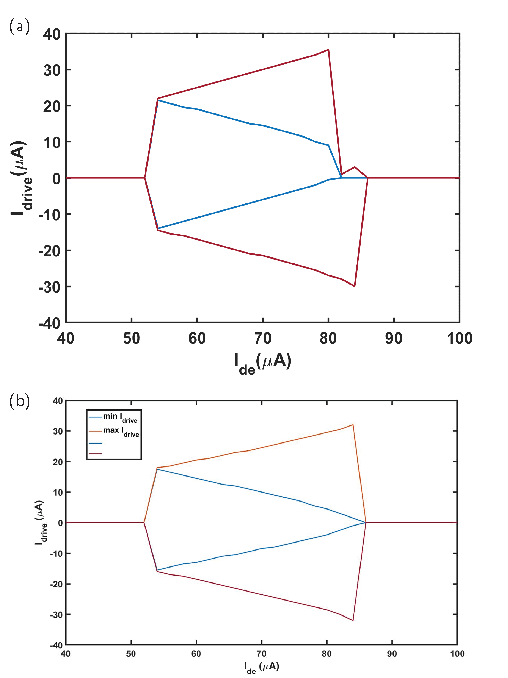
\includegraphics[width=8.6cm]{figures/_fig__dendrites__min_max__4jj.pdf}
%\captionof{figure}{\label{fig:dendrites_min_max__4jj}Caption of fig:dendrites min max 4jj.}
%\end{figure}

\subsection{\label{apx:neuronal_thresholding}Details regarding neuronal thresholding}
\begin{equation}
\label{eq:neuronal_thresholding}
\begin{split}
\frac{dI^{\mathrm{th}}_2}{dt} = & - \frac{r}{L^{\mathrm{th}}_{\mathrm{t}}} + \frac{M^{\mathrm{\mathrm{nt}}|\mathrm{ni}}}{L^{\mathrm{nt}}_{\mathrm{t}}} \frac{dI^{\mathrm{ni}}}{dt} \\
& - \frac{ M^{\mathrm{nt}|\mathrm{nr}} M^{\mathrm{\mathrm{nr}}|\mathrm{si}} }{ L^{\mathrm{nr}}_{\mathrm{t}} L^{\mathrm{nt}}_{\mathrm{t}} } \frac{dI^{\mathrm{si}}}{dt}.
\end{split}
\end{equation}

\section{\label{apx:hTron}hTron model}

\

\section{\label{apx:fan_in}Analysis of dendritic and neuronal fan-in}

Fan-out and fan-in are primary considerations of neuronal circuits when assessing scaling potential. Consideration of fan-out has led to the proposal for photonic communication, which we have addressed in prior studies \cite{shbu2017,chbu2017,chbu2018,sh2018_ICRC,sh2019,sh2020}. The present study relates to models of dendrites and neurons, which perform fan-in through the synapto-dendritic tree. Analysis of the number of input connections to a dendrite or neuron cell body are therefore necessary to complete the study.

\begin{figure}[h!]
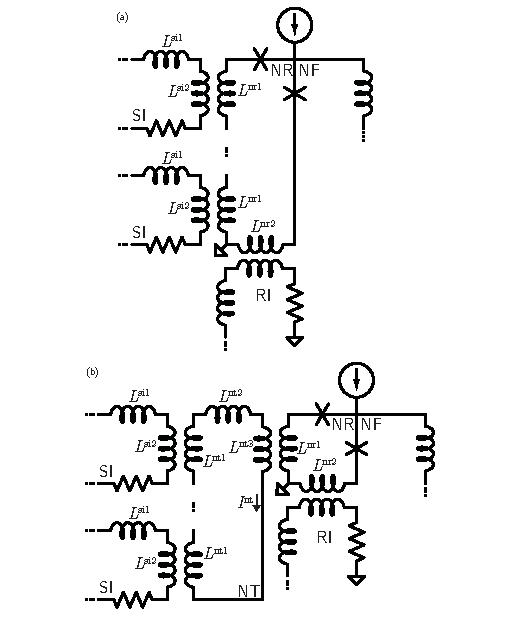
\includegraphics[width=8.6cm]{figures/_fig_apx__fan-in__circuits.pdf}
\captionof{figure}{\label{fig:fan-in__circuits}Caption of fig:fan-in circuits.}
\end{figure}
For synaptic or dendritic integration loops coupled directly to a dendritic or neuronal receiving loop, we would like to know how to choose the inductors shown in Fig.\,\ref{fig:fan-in__circuits}(a) so the applied flux stays in the appropriate operating range as the number of synaptic connections, $N$, is modified. This consideration will identify the limit of how many synapses can be coupled to a single dendrite or neuron\textemdash the fan-in limit. 

We have seen that the operation of a dendrite (or neuron cell body) is significantly shaped by the inductance of the DR loop. We would therefore like to be able to increase the number of synaptic connections without changing the total inductance of this loop. This total inductance is given by
\begin{equation}
\label{eq:fan-in__direct_input__si_inductance}
L^{\mathrm{nr1}}_{\mathrm{tot}} = \sum_i L^{\mathrm{nr1}}_i = N L^{\mathrm{nr1}}_0
\end{equation}
We would like $L^{\mathrm{nr1}}_{\mathrm{tot}}$ to be independent of $N$, which is possible with $L^{\mathrm{nr1}}_N = L^{\mathrm{nr1}}_0/N$. The total applied flux to the NR loop is given by
\begin{equation}
\label{eq:fan-in__direct_input__applied_flux}
\Phi_{\mathrm{a}}^{\mathrm{nr}} = \sum_i M_i^{\mathrm{si|nr}} \, I_i^{\mathrm{si}}.
\end{equation}
Suppose all SI loops contain a given current, $I_0^{\mathrm{si}}$. We would like the applied flux to the NR loop, $\Phi_{\mathrm{a}}^{\mathrm{nr}}$, to be independent of $N$:
\begin{equation}
\label{eq:fan-in__direct_input__flux_independent_of_N}
\frac{ \Phi_{\mathrm{a}}^{\mathrm{nr}} }{ I_0^{\mathrm{si}} } = \mathrm{cnst.} \neq f(N).
\end{equation}
In the case where all mutual inductors between synapses and the NR loop are equal,
\begin{equation}
\label{eq:fan-in__direct_input__flux_independent_of_N_2}
\frac{ \Phi_{\mathrm{a}}^{\mathrm{nr}}(N) }{ I_0^{\mathrm{si}} } = N\,k\,\sqrt{ L_N^{\mathrm{si2}} \, L_N^{\mathrm{nr1}}},
\end{equation}
where $L_N^{\mathrm{si2}}$ and $L_N^{\mathrm{nr1}}$ are the values of $L^{\mathrm{si2}}$ and $L^{\mathrm{nr1}}$ that we should choose for the SI loop output inductor when there are $N$ synapses coupled directly to the NR loop. We have seen above that we need $L_N^{\mathrm{nr1}} = L_0^{\mathrm{nr1}}/N$ to maintain the inductance of the NR loop. Therefore, in order for Eq.\,\ref{eq:fan-in__direct_input__flux_independent_of_N_2} to satisfy Eq.\,\ref{eq:fan-in__direct_input__flux_independent_of_N}, we must also have $L_N^{\mathrm{si2}} = L_0^{\mathrm{si2}}/N$.

This consideration does not explicitly identify a fan-in limit. This limit arises due to practical considerations related to making $L^{\mathrm{si2}}$ and $L^{\mathrm{nr1}}$ exceedingly small as $N$ grows large. Taking $L_0 \approx 1$\,pH as a rough lower limit on what we would like to fabricate, and $L_{\mathrm{tot}}^{\mathrm{nr}} \approx 20$\,pH, we see direct fan-in with this circuit design is limited to about 20. This limit can be straightforwardly overcome with an intermediate transformer collection coil, as shown in Fig.\,\ref{fig:fan-in__circuits}(b). In this configuration, the applied flux to the NR loop is
\begin{equation}
\label{eq:fan-in__transformer_collection__full}
\Phi_{\mathrm{a}}^{\mathrm{nr}} = \frac{ M^{\mathrm{nr|nt}} \, \sum_i M^{\mathrm{nt|si}}_i I_i^{\mathrm{si}} }{ \sum_i L^{\mathrm{nt1}}_i + L^{\mathrm{nt2}} + L^{\mathrm{nt3}} }.
\end{equation}
The mutual inductors are $M^{\mathrm{si|nt}} = k\sqrt{L^{\mathrm{si2}} \, L^{\mathrm{nt1}}}$ and $M^{\mathrm{nt|nr}} = k\sqrt{L^{\mathrm{nt3}} \, L^{\mathrm{nr1}}}$. We are interested in how this flux scales with the number $N$ of input synapses to the neuronal transformer (NT) loop. Consider the case where the mutual inductors between all synapses and the NT loop are identical: $M^{\mathrm{nt|si}}_i = M^{\mathrm{nt|si}} = k \sqrt{L^{\mathrm{si2}}L^{\mathrm{nt1}}}$, and $L^{\mathrm{nt1}}_i = L^{\mathrm{nt1}}$. Further assume all synaptic integration loops carry the same current $I^{\mathrm{si}}_i = I^{\mathrm{si}}_0$. Such a case is rare in operation but is sufficient for scaling analysis. Equation \ref{eq:fan-in__transformer_collection__full} becomes
\begin{equation}
\label{eq:fan-in__transformer_collection__identical_synapses}
\frac{ \Phi_{\mathrm{a}}^{\mathrm{nr}} }{ I^{\mathrm{si}}_0 } = \frac{ M^{\mathrm{nr|nt}} \, M^{\mathrm{nt|si}} }{ L^{\mathrm{nt1}} } \left( 1 + \frac{ L^{\mathrm{nt2}} + L^{\mathrm{nt3}} } { N L^{\mathrm{nt1}} } \right)^{-1}.
\end{equation}
From Eq.\,\ref{eq:fan-in__transformer_collection__identical_synapses} one can see the ratio of flux in the NR loop to current in each of the SI loop becomes nearly independent of $N$ for large $N$. 

We can further elucidate the scaling by noting that the circuit of Fig.\,\ref{fig:fan-in__circuits}(b) has three types of inductors. Transformers are likely to be asymmetrical, with a larger inductor coupling flux into a smaller inductor to achieve a reasonable mutual inductance with a modest receiving loop inductance. We can therefore specify $M^{\mathrm{nr|nt}} = M^{\mathrm{nt|si}} = k \sqrt{ L_{\mathrm{m}} \, L_{\mathrm{s}}}$, where $L_{\mathrm{m}}$ refers to a medium-sized inductor, on the order of 100\,pH, and $L_{\mathrm{s}}$ is a small inductor, on the order of 10\,pH. Thus, $L^{\mathrm{si2}} = L^{\mathrm{nt3}} = L_{\mathrm{m}}$, and $L^{\mathrm{nt1}} = L^{\mathrm{nr1}} = L_{\mathrm{s}}$. The inductor $L^{\mathrm{nt2}}$ is a parasitic inductance that we anticipate being unavoidable in the fabrication of a large NT loop. We assume $L^{\mathrm{nt2}} = L_{\mathrm{m}}$. The third inductance in the circuit is $L^{\mathrm{si1}}$, a large self-inductance unassociated with a transformer, which we label as a big inductor, $L_{\mathrm{b}}$. This inductance will likely be in the range of 10\,nH - 10\,\textmu H, and for the sake of this analysis consideration of the value of 10\,nH is sufficient. The large value of this inductance gives the synapse (or dendrite in the case of a DI loop) an analog response. In hardware, such large values are made possible by high-kinetic-inductance materials \cite{}, wherein the inductance is a result of the motion of the current-carrying cooper pairs rather than the coupling between a current and the magnetic field it produces. With these simplifications, Eq.\,\ref{eq:fan-in__transformer_collection__identical_synapses} becomes
\begin{equation}
\label{eq:fan-in__transformer_collection__three_inductances}
\frac{ \Phi_{\mathrm{a}}^{\mathrm{nr}} }{ I^{\mathrm{si}}_0 } = k^2 L_{\mathrm{m}} \left( 1 + \frac{2L_{\mathrm{m}}}{NL_{\mathrm{s}}} \right)^{-1}.
\end{equation}
The term $2L_{\mathrm{m}}/NL_{\mathrm{s}}$ is of order unity when $N\approx 10$ and becomes small when $N \approx 100$. In the large-$N$ limit we can make the approximation
\begin{equation}
\label{eq:fan-in__transformer_collection__large_N}
\frac{ \Phi_{\mathrm{a}}^{\mathrm{nr}} }{ I^{\mathrm{si}}_0 } \approx k^2 L_{\mathrm{m}} \left( 1 - \epsilon \right) + \mathcal{O}(\epsilon^2),
\end{equation}
where
\begin{equation}
\label{eq:fan-in__transformer_collection__epsilon}
\epsilon \equiv \frac{ 2L_{\mathrm{m}} }{ N L_{\mathrm{s}} }.
\end{equation}
Thus, a dendrite or neuron receiving input from $N$ synapses or dendrites, each containing current $I^{\mathrm{si}}_0$ in their integration loop, receives flux that is independent of $N$ to leading order. This appears to be an advantageous fan-in scenario, made possible by the shared transformer collection coil. We have seen above that roughly 20 synapses or dendrites can be directly coupled to a receiving loop. When 20 synapses or dendrites are coupled to a transformer collection coil, $\epsilon$ is on the order of unity, and therefore not sufficiently small as to be neglected for design purposes. Yet in this case the total applied flux to the receiving loop will be within a factor of two of the directly coupled case. Above 20 inputs, the situation only improves with $N$. Therefore, it appears fan-in is achievable for any number of inputs. 

To gain further confidence in this conclusion, we must consider the ability of a collection of $N$ inputs to drive a dendrite or neuron to threshold as well as the cross talk between the inputs. Let us refer to the value of flux that will drive the neuron above threshold as $\Phi^{\mathrm{nr}}_{\mathrm{th}}$. As discussed in Sec.\,\ref{sec:dendrites}, this value is determined by circuit parameters and current biases, which are independent of the number of inputs. As a model of scaling potential, we would like to know what value of $I^{\mathrm{si}}_{\mathrm{th}}$ is required in each synapse of a homogeneous point neuron to achieve $\Phi^{\mathrm{nr}}_{\mathrm{th}}$. In the large-$N$ limit, we can straightforwardly rearrange Eq.\,\ref{eq:fan-in__transformer_collection__large_N} and apply the binomial approximation to arrive at
\begin{equation}
\label{eq:fan-in__transformer_collection__threshold_current}
I^{\mathrm{nr}}_{\mathrm{th}} = \frac{1+\epsilon}{k^2 L_{\mathrm{m}}} \Phi^{\mathrm{nr}}_{\mathrm{th}}.
\end{equation}
Again we find the quantity of interest is independent of $N$ to leading order. The factor proportional to $\epsilon$ must be accounted for in design, but the scaling with large $N$ is favorable. 

Consider the smallest number of synapses capable of achieving the threshold flux. There are $N$ synapses on the transformer collection coil, and we seek the number $P$ of them such that when those synapses reach saturation ($I^{\mathrm{si}} = I^{\mathrm{si}}_{\mathrm{sat}}$) the total applied flux reaches threshold ($\Phi^{\mathrm{nr}}_{\mathrm{a}} = \Phi^{\mathrm{nr}}_{\mathrm{th}}$). Here we begin with the exact expression of Eq.\,\ref{eq:fan-in__transformer_collection__full} rather than making a large-$N$ approximation. Assuming again identical synapses, and taking inductors to be small ($L_{\mathrm{s}}$), medium ($L_{\mathrm{m}}$), or big ($L_{\mathrm{b}}$), we can calculate the fraction of saturated synapses required to reach threshold, assuming all other synapses have zero integrated current.
\begin{equation}
\label{eq:fan-in__transformer_collection__fraction_for_threshold}
\frac{P}{N} = \frac{ \Phi^{\mathrm{nr}}_{\mathrm{th}} }{ k^2  I^{\mathrm{si}}_{\mathrm{sat}} } \left( \frac{1}{ L_{\mathrm{m}} } + \frac{2}{ N L_{\mathrm{s}} }  \right).
\end{equation}
The leading term is again independent of $N$, and the correction term recedes as $1/N$. The fraction of synapses that must be active to drive a dendrite or neuron above threshold converges to a fixed value at large $N$. Using realistic numbers, in the small-$N$ limit, $P/N \approx 0.1$, and in the large-$N$ limit, $P/N \approx 0.03$.

Finally, we consider cross talk between synapses or dendrites coupled to a common transformer receiving loop. Consider an NT loop with $N$ synaptic connections, $n$ of which contain current $I^{\mathrm{si}}_0$ in their SI loop. A net current will be induced in the NT loop due to the flux from the synapses,
\begin{equation}
\label{eq:fan-in__transformer_collection__I_nt}
I^{\mathrm{nt}} = \frac{\Phi^{\mathrm{nt}}}{L^{\mathrm{nt}}}\rightarrow \frac{ n k \sqrt{L_{\mathrm{m}}\,L_{\mathrm{s}}}}{NL_{\mathrm{s}}+2L_{\mathrm{m}}},
\end{equation}
and this current will induce a current in each SI loop, $I^{\mathrm{si}}_{\mathrm{ind}} = \Phi^{\mathrm{si}}_{\mathrm{ind}}/L^{\mathrm{si}} = M^{\mathrm{si|nt}}I^{\mathrm{nt}}/(L^{\mathrm{si1}}+L^{\mathrm{si2}})$. Making the association $L^{\mathrm{si1}} = L_{\mathrm{b}}$, and approximating $L_{\mathrm{b}} + L_{\mathrm{m}} \approx L_{\mathrm{b}}$, we find the ratio of the induced current in each SI loop to the integrated current in one of the $P$ active synapses is
\begin{equation}
\label{eq:fan-in__transformer_collection__cross_talk}
\frac{I^{\mathrm{si}}_{\mathrm{ind}}}{I^{\mathrm{si}}_0} = \frac{n}{N}\frac{k^2L_{\mathrm{m}}}{L_{\mathrm{b}}}\left( 1+\epsilon \right)^{-1}.
\end{equation}
As stated above, $L_{\mathrm{b}}$ is likely to be in the range of 10\,nH - 10\,\textmu H, while $L_{\mathrm{m}}$ is on the order of 100\,pH. The term $L_{\mathrm{m}}/L_{\mathrm{b}}$ will be less than 0.01, and typically much less than this value. The worst case for cross talk occurs when all synapses contain integrated current $I^{\mathrm{si}}_0$ so $n = N$. For rough estimate of scaling, we can ignore the $k^2$ term and the $\epsilon$ term, both of which act to reduce the cross talk. In the extreme limit where all $N$ SI loops contain the saturated current $I^{\mathrm{si}}_{\mathrm{sat}}$, the fraction of current induced in each loop scales as
\begin{equation}
\label{eq:fan-in__transformer_collection__cross_talk__worst_case}
\frac{I^{\mathrm{si}}_{\mathrm{ind}}}{I^{\mathrm{si}}_{\mathrm{sat}}} \approx \frac{L_{\mathrm{m}}}{L_{\mathrm{b}}}.
\end{equation}
The key feature of loop neurons regarding cross talk is that the SI loop inductance is large, yet a small fraction of this inductance feeds into the mutual inductor. The asymmetry of the inductances between $L^{\mathrm{dr}}$ and $L^{\mathrm{di}}$ is necessary to reduce cross talk. This inductance imbalance is also precisely what enables the dendrite to produce an analog output. If one uses a dendrite or neuron to produce a binary, single-flux-quantum output, the inductance of the DI loop will be on the same order as the inductance of the inductors in the transformers, and cross talk will cause a problem for fan-in. However, leveraging high-kinetic-inductance materials and analog synapses and dendrites, cross talk is not a problem, and fan-in behaves favorably from a small number of inputs up to large $N$.

\bibliographystyle{unsrt}
\bibliography{phenomenological_modeling}

\end{document}